\chapter{Pruebas y resultados}
	En este apartado se muestran las pruabsa y resultados del funcionamiento del sistema, las cuales ser\'an organizadas por m\'odulo.\\

	Los modulos que se someter\'an a revisi\'on son los siguientes:
	\begin{itemize}
		\item Departamentos.
		\item F\'ormulas.
		\item Grupos de f\'ormulas.
		\item Proceso.
	\end{itemize}

	Las pruebas que se realizaran son las siguientes:
	\begin{itemize}
		\item Visualizaci\'on del m\'odulo y su respectiva informaci\'on.
		\item Creaci\'on de un nuevo registro.
		\item Eliminaci\'on de un nuevo registro.
		\item Actualizaci\'on de un registro existente.
		\item Acciones adicionales en caso de que existan.
	\end{itemize}

	A continuaci\'on se procede a mostrar las pruebas de los m\'odulos. 

	\section{Pruebas y resultados de las p\'aginas principales del SII.}

		Como primera prueba se realizara la ejecuci\'on de la p\'agina principal del sistema, la cual se muestra en la figura \ref{fig_principal}

		\begin{figure}[H]
	        \centering
	        
\includegraphics[width=16cm, height=9.5cm]{figuras/principal}
	        \caption{Pantalla de inicio del Sisitema Integral de Informaci\'on del ITT.}
	        \label{fig_principal}
	    \end{figure}

	    En esta pantalla se pueden visualizar las diferentes opciones que tendr\'a el sistema, en esta ocasi\'on el \'unico con funcionalidad es el de indicadores. Estas funcionalidades se mostraran en un futuro dependiendo del tipo de usuario que ingrese al sistema, ya que en este caso los indicadores, solamente podr\'an ser visualizados por personal autorizado.\\

	    Para entrar a las opciones permitidas en los indicadores se tiene que dar click el el bot\'on con la leyenda ``indicadores" que se encuentra en el men\'u principal mostrando la pantalla que se muestra en la figura \ref{fig_principali}.\\

	    Esta pantalla muestra dos funcionalidades las cuales son:
	    \begin{itemize}
	    	\item \textbf{Configuraci\'on:} Pantalla con las opciones para configurar las funciones y datos necesarias para realizar un periodo de indicadores.
	    	\item \textbf{Proceso:} Pantalla con todas las funcionalidades para consultar y procesar los periodos de indicadores.
	    \end{itemize}


	    \begin{figure}[]
	        \centering
	        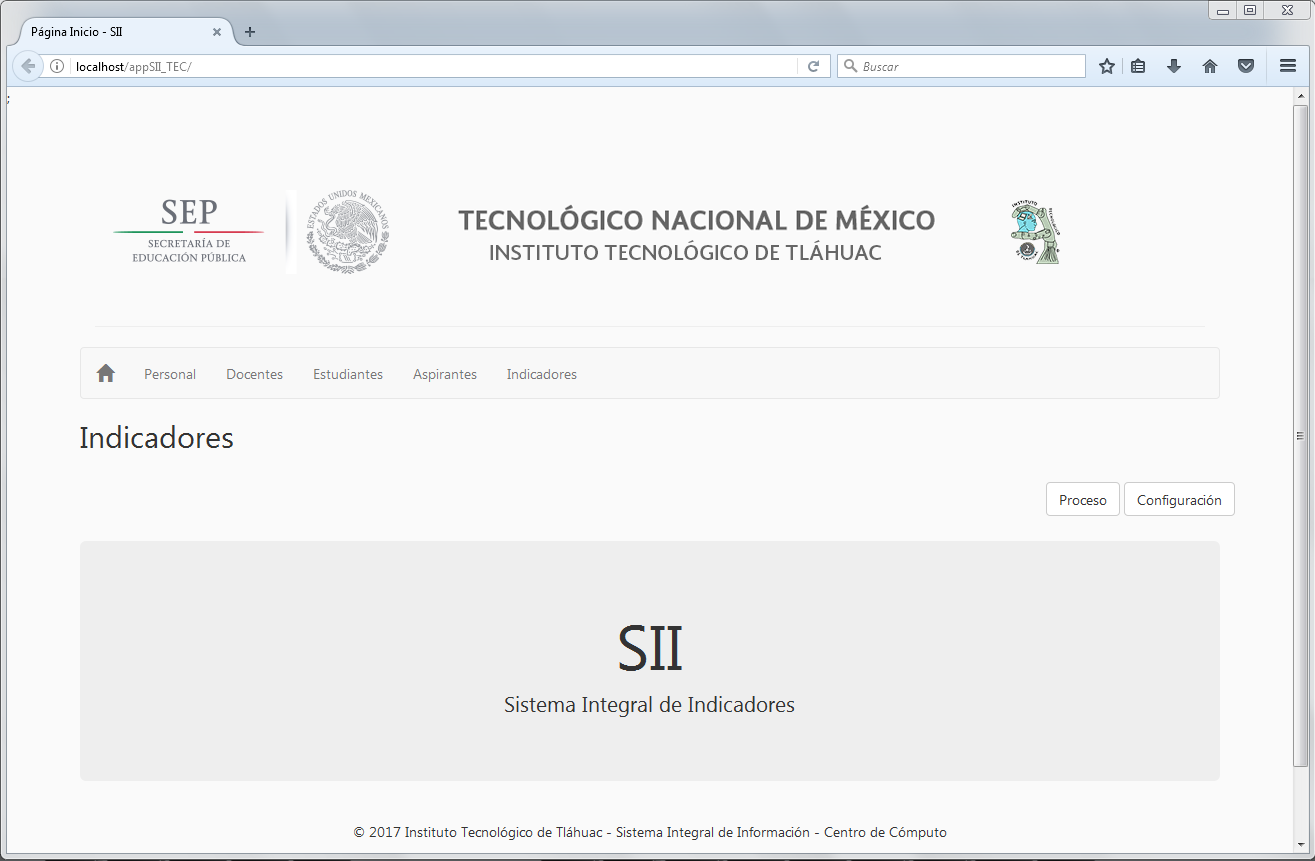
\includegraphics[width=16cm, height=9.5cm]{figuras/principali}
	        \caption{Pantalla de inicio del Sisitema Integral de Indicadores.}
	        \label{fig_principali}
	    \end{figure}

		\section{Pruebas y resultados de m\'odulo Departamentos.}

			Para ingresar al m\'odulo de configuraci\'on de departamentos, es necesario dar click en el bot\'on Configuraci\'on $\rightarrow$  Departamentos, lo cual nos mostrara la ventana ilustrada en la figura \ref{fig_Departamentos}.

			\begin{figure}[H]
		        \centering
		        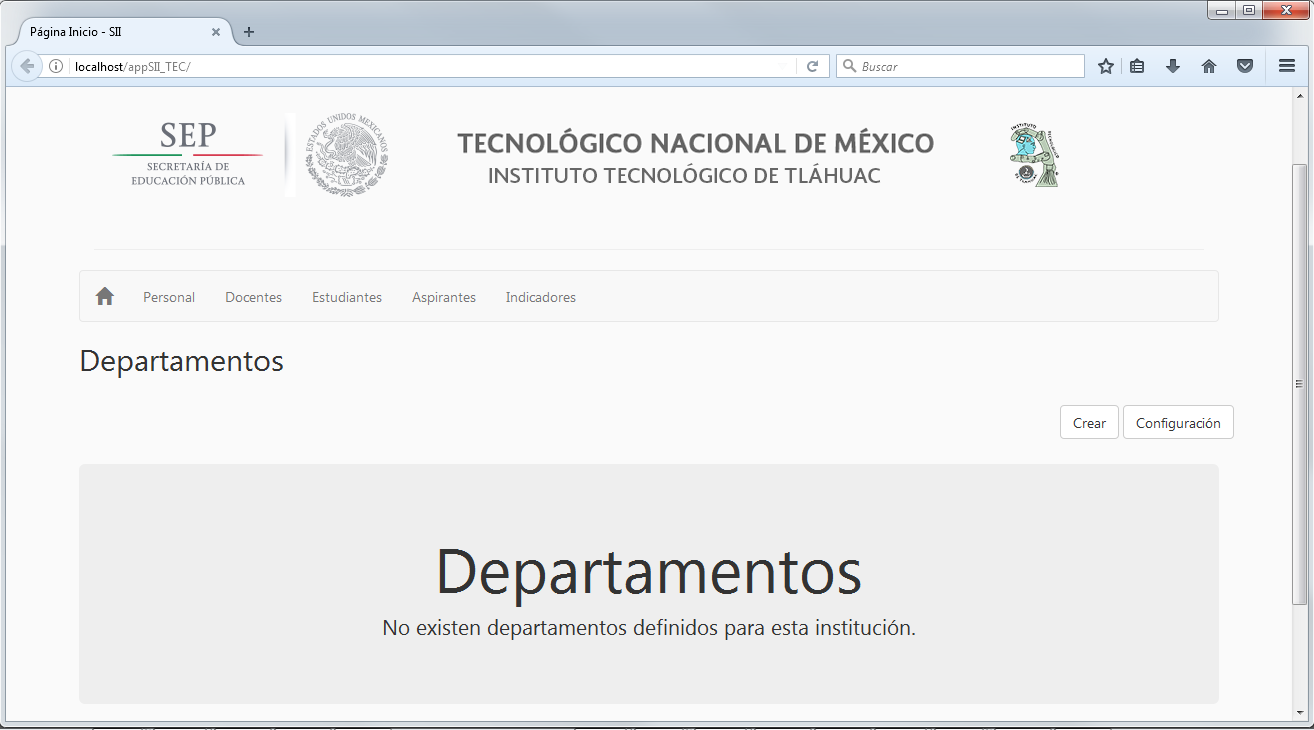
\includegraphics[width=16cm, height=9.5cm]{figuras/Departamentos}
		        \caption{Pantalla principal de departamentos.}
		        \label{fig_Departamentos}
		    \end{figure}

			El m\'odulo de departamentos cuenta con las siguientes funciones para validar:
			\begin{itemize}
				\item Alta de departamento.
				\item Actualizaci\'on de departamentos.
				\item Baja de departamentos.
			\end{itemize}

			Estas acciones se muestran a continuaci\'on:

			\subsection{Alta de departamento}

			Para crear un departamento, se tiene que dar click en el bot\'on crear del m\'odulo de configuraci\'on de departamentos, mostrando con esto la ventana emergente  que se puede ver en la figura \ref{fig_DepartamentosCrear}.

			\begin{figure}[H]
		        \centering
		        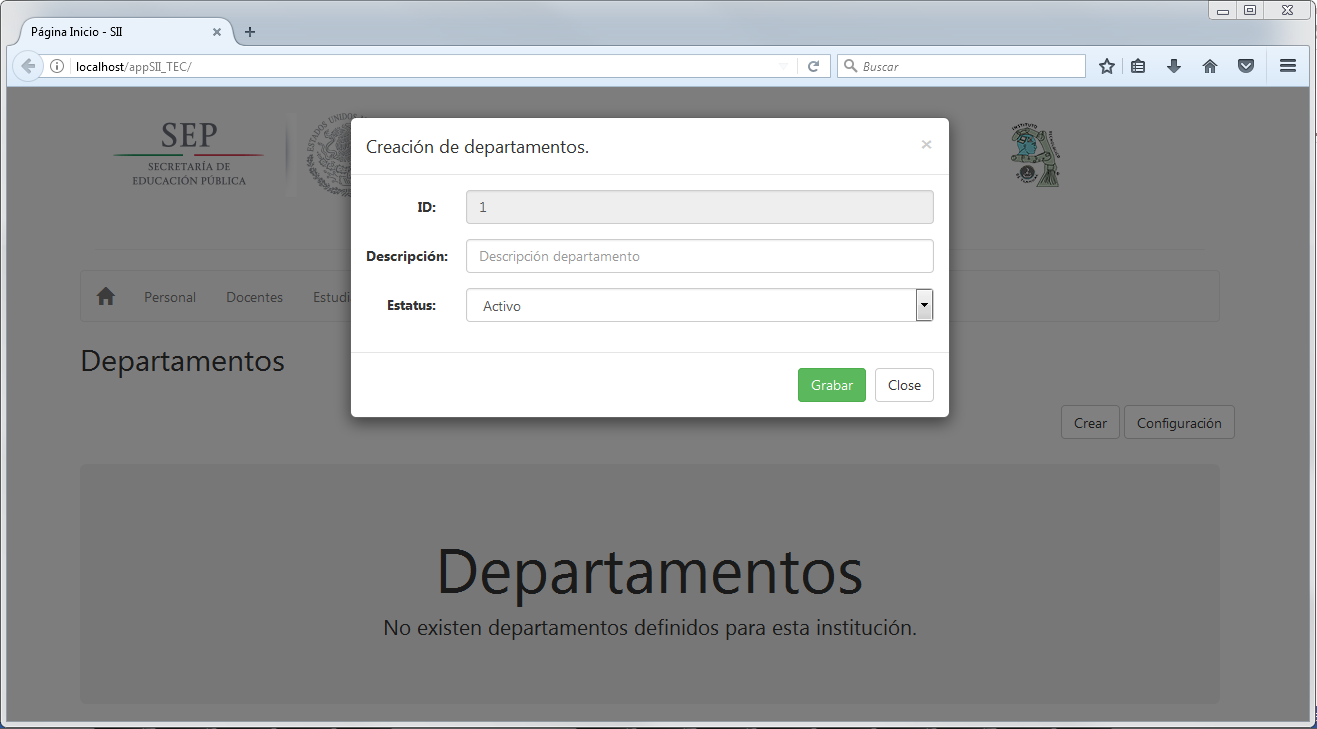
\includegraphics[width=16cm, height=9.5cm]{figuras/DepartamentosCrear}
		        \caption{Ventana emergente para creaci\'on de departamentos.}
		        \label{fig_DepartamentosCrear}
		    \end{figure}
			
			Los datos que se solicitan para la creaci\'on de un departamento son los siguientes:
			\begin{enumerate}[1.]
				\item \textbf{ID:} N\'umero identificador, este se genera de manera autom\'atica, es por esto que se muestra deshabilitado.
				\item \textbf{Descripci\'on:} Campo para almacenar una breve descripci\'on del departamento.
				\item \textbf{Estatus:} Campo para indicar si el departamento es activo o no.
			\end{enumerate}

			Cuando uno de estos datos no se ingresa correctamente, se muestra un mensaje de error tal como se muestra en la figura \ref{fig_DepartamentosValida}.

			\begin{figure}[H]
		        \centering
		        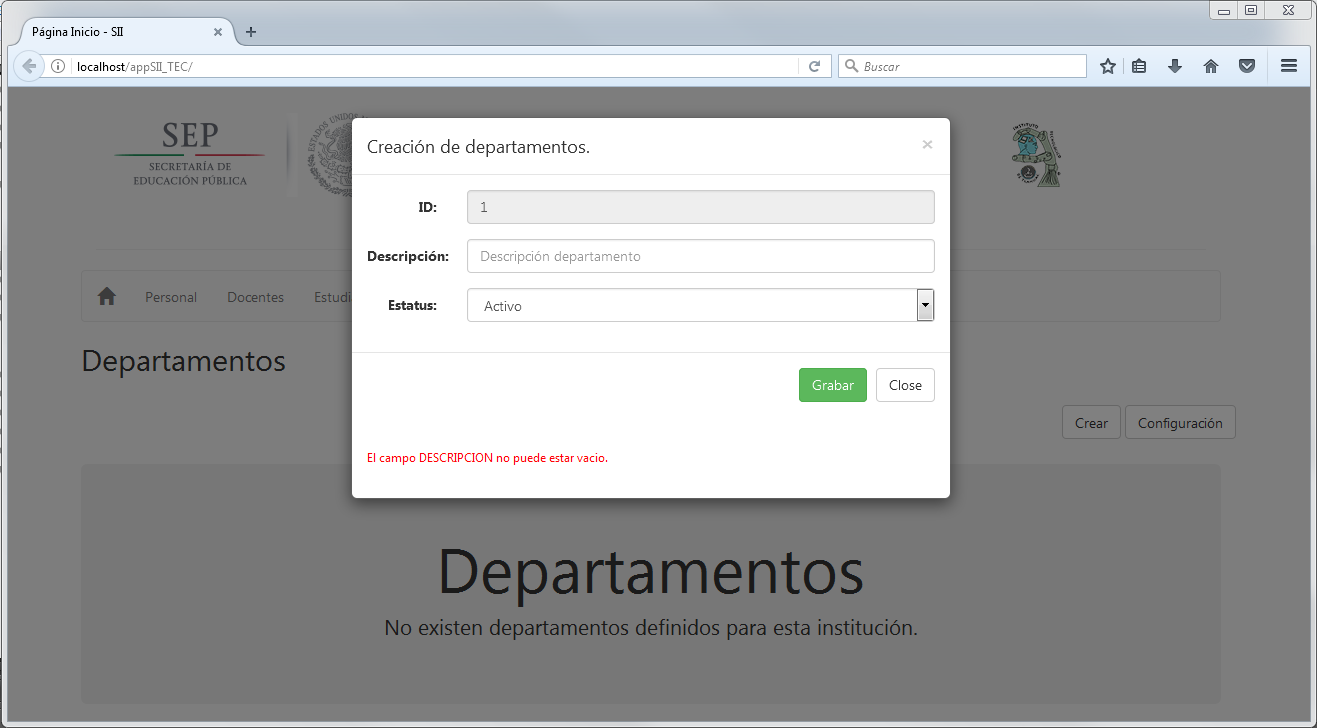
\includegraphics[width=16cm, height=9.5cm]{figuras/DepartamentosValida}
		        \caption{Mensaaje de validaci\'on departamentos.}
		        \label{fig_DepartamentosValida}
		    \end{figure}

		    Al momento de ingresar los datos correctamente, el sistema graba el registro en la base de datos y manda un mensaje indicando que el proceso se realiz\'o correctamente, esto se muestra en la figura \ref{img_DepartamentoGraba}.\\

		    \begin{figure}[]
		        \centering
		        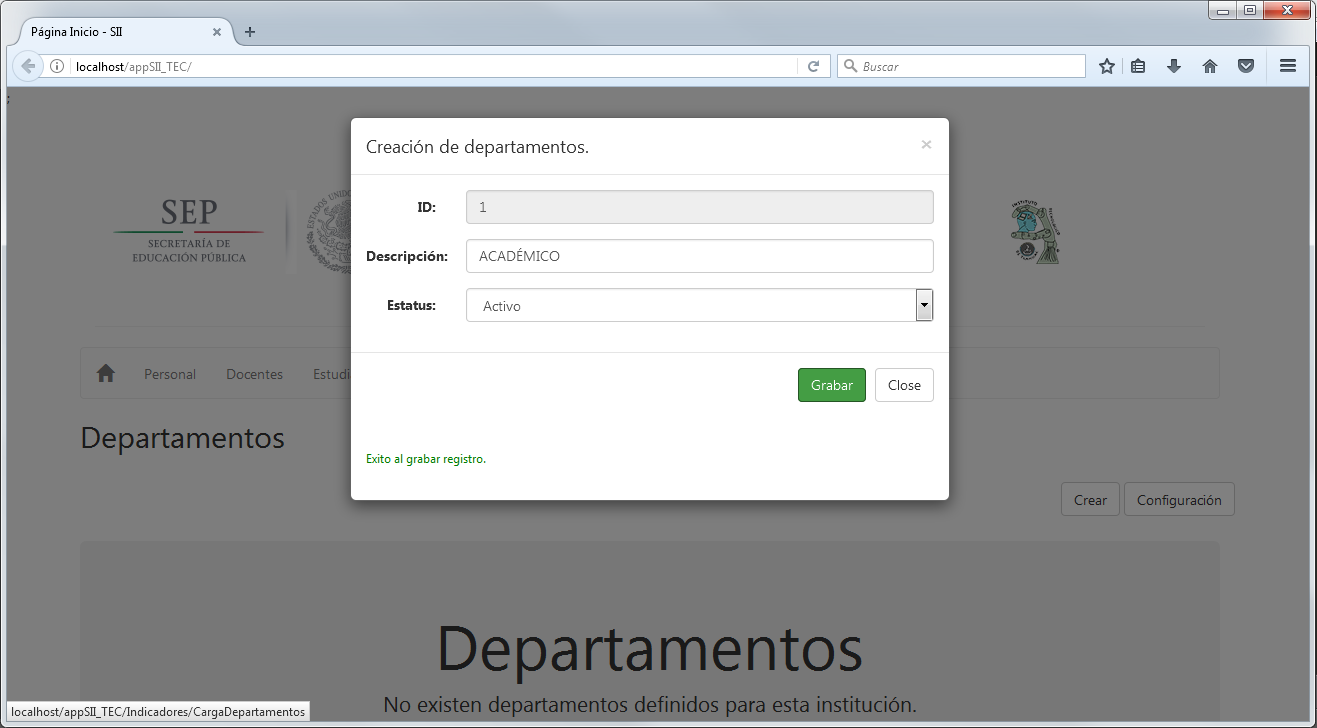
\includegraphics[width=16cm, height=9.5cm]{figuras/DepartamentosGraba}
		        \caption{Mensaaje de grabaci\'on satisfactoria de departamento.}
		        \label{img_DepartamentoGraba}
		    \end{figure}

		    Una vez que existen departamentos registrados en la base de datos, estos se muestran en una tabla, la cual tendr\'a dos acciones espec\'ificas por departamento, una es actualizar y la otra es eliminar. Esta tabla de departamentos se muestra en la figura \ref{fig_DepartamentoTabla}.\\

		    \begin{figure}[]
		        \centering
		        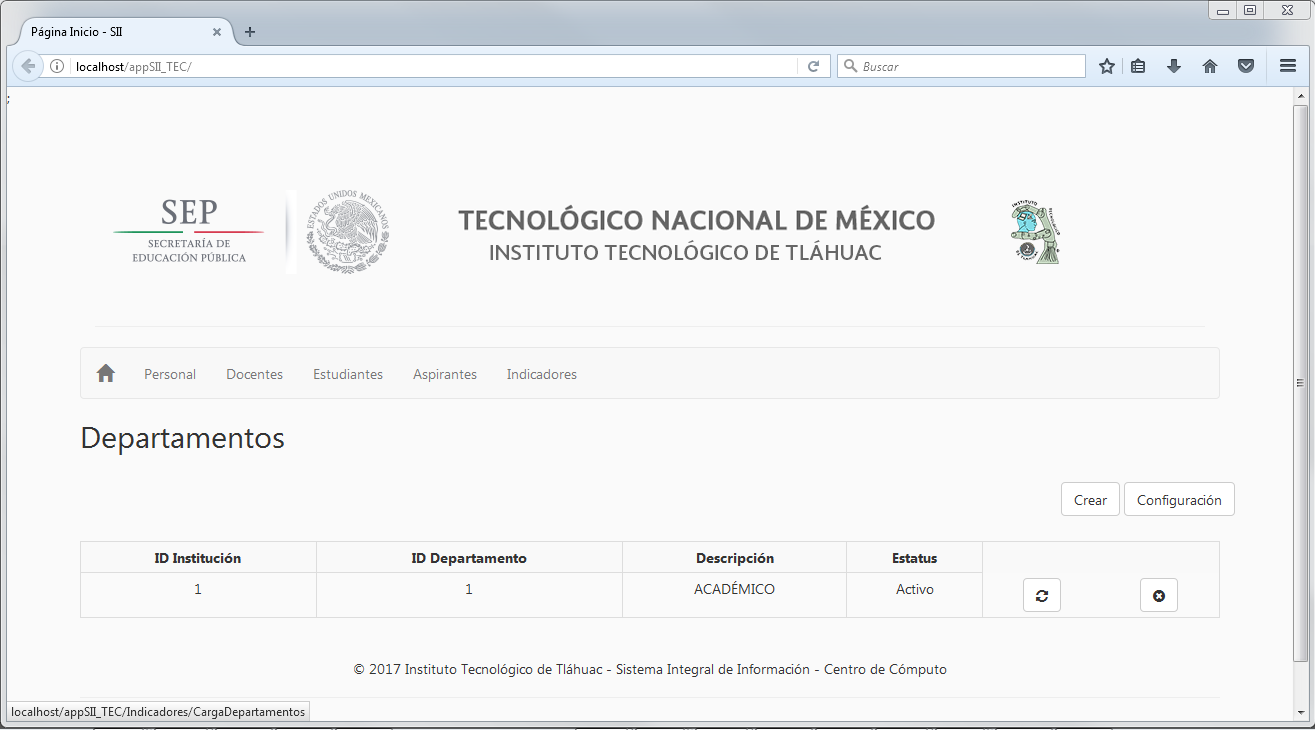
\includegraphics[width=16cm, height=9.5cm]{figuras/DepartamentosTabla}
		        \caption{Listado de departamentos.}
		        \label{fig_DepartamentoTabla}
		    \end{figure}
			
			\subsection{Actualizaci\'on de departamentos}

			Para la actualizaci\'on de departamentos se muestra la misma ventana emergente que se usa para crear uno, pero en este caso se visualizan los datos del departamento que se seleccion\'o. En este caso se muestra la ventana emergente en la que se quiere actualizar el departamento acad\'emico, esta ventana se muestra en la figura \ref{fig_DepartamentoActualiza}.

			\begin{figure}[]
		        \centering
		        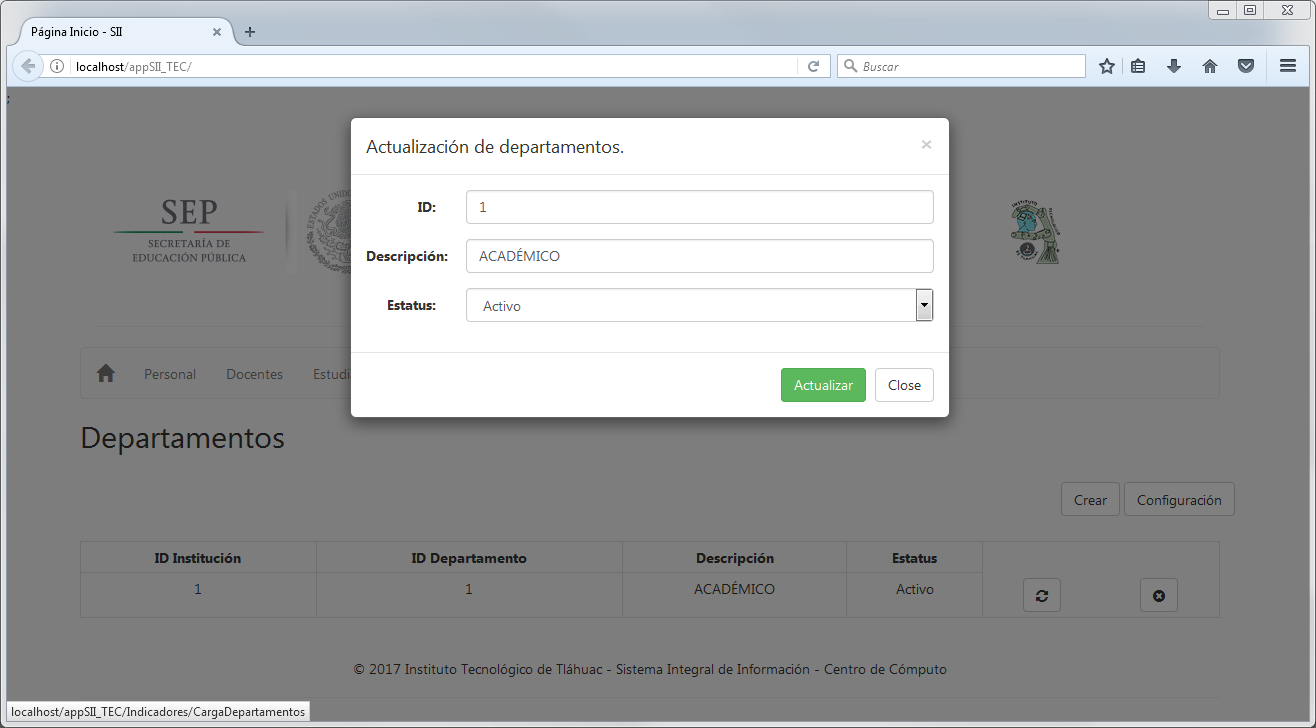
\includegraphics[width=16cm, height=9.5cm]{figuras/DepartamentosActualiza}
		        \caption{Ventana emergente de actualizaci\'on de departamento.}
		        \label{fig_DepartamentoActualiza}
		    \end{figure}

		    \subsection{Baja de departamentos}

		    Como \'ultima prueba se muestra en la figura \ref{fig_DepartamentoElimina} la ventana emergente mostrada al momento de querer eliminar un departamento, el sistema pregunta que el usuario este seguro de eliminar este registr\'o.\\\\\\\\\\

		    \begin{figure}[]
		        \centering
		        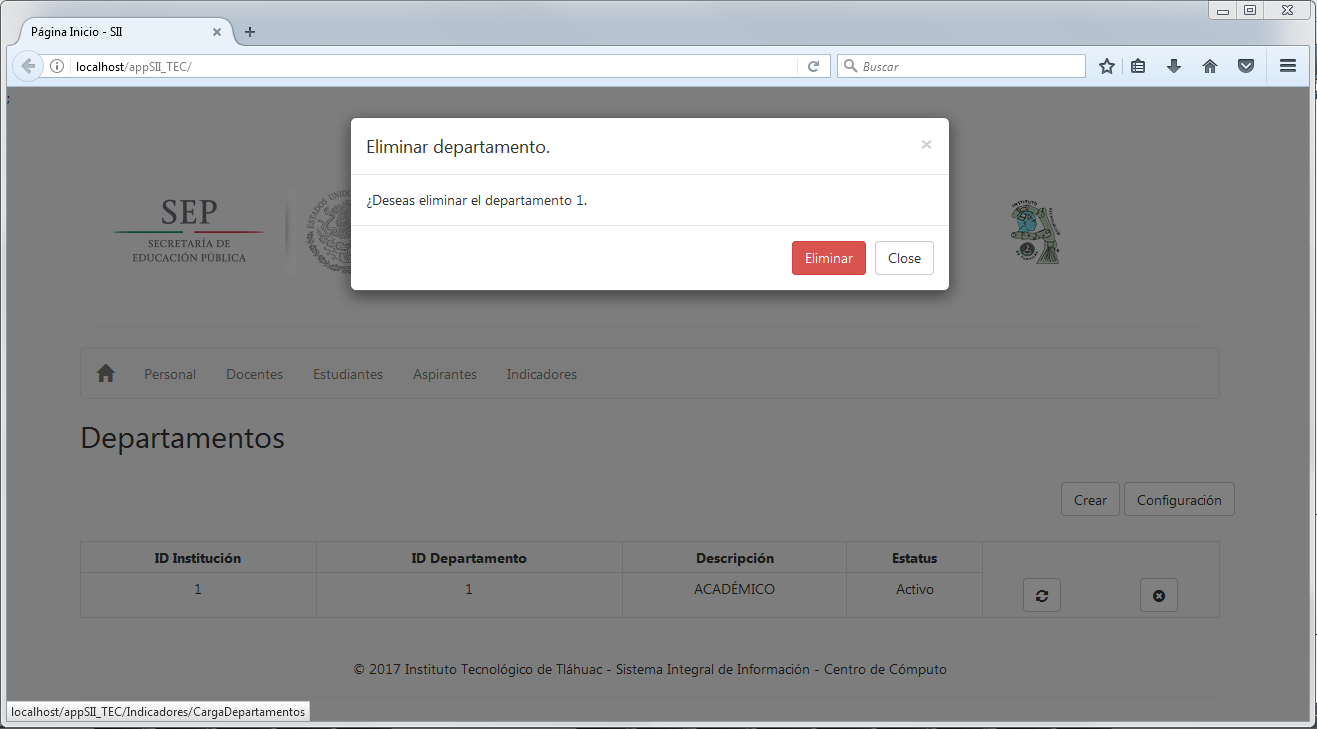
\includegraphics[width=16cm, height=9.5cm]{figuras/DepartamentosElimina}
		        \caption{Mensaje de advertencia al eliminar departamento.}
		        \label{fig_DepartamentoElimina}
		    \end{figure}








		\section{Pruebas y resultados de m\'odulo F\'ormulas.}

			Para ingresar al m\'odulo de configuraci\'on de f\'ormulas, es necesario dar click en el bot\'on Configuraci\'on $\rightarrow$ Formulas, lo cual nos mostrara la ventana ilustrada en la figura \ref{fig_Formulas}.


			\begin{figure}[H]
		        \centering
		        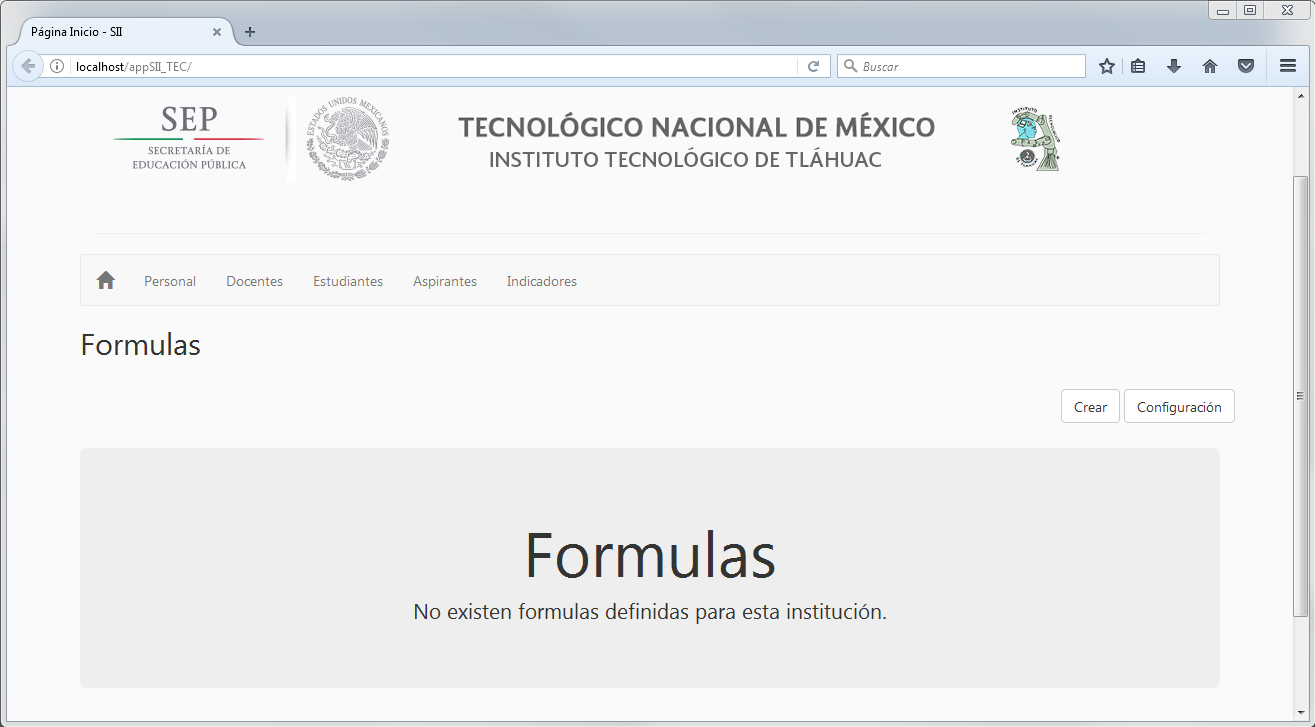
\includegraphics[width=16cm, height=9.5cm]{figuras/Formulas}
		        \caption{Pantalla principal de f\'ormulas.}
		        \label{fig_Formulas}
		    \end{figure}
			
			El m\'odulo de f\'ormulas cuenta con las siguientes funciones para validar:
			\begin{itemize}
				\item Alta de f\'ormulas.
				\item Actualizaci\'on de f\'ormulas.
				\item Baja de f\'ormulas.
			\end{itemize}

			Estas acciones se muestran a continuaci\'on:

			\subsection{Alta de f\'ormula}

			Para crear una f\'ormula, se tiene que dar click en el bot\'on crear del m\'odulo de configuraci\'on de f\'ormulas, mostrando con esto la ventana emergente  que se puede ver en la figura \ref{fig_FormulasCrear}.\\

			\begin{figure}[]
		        \centering
		        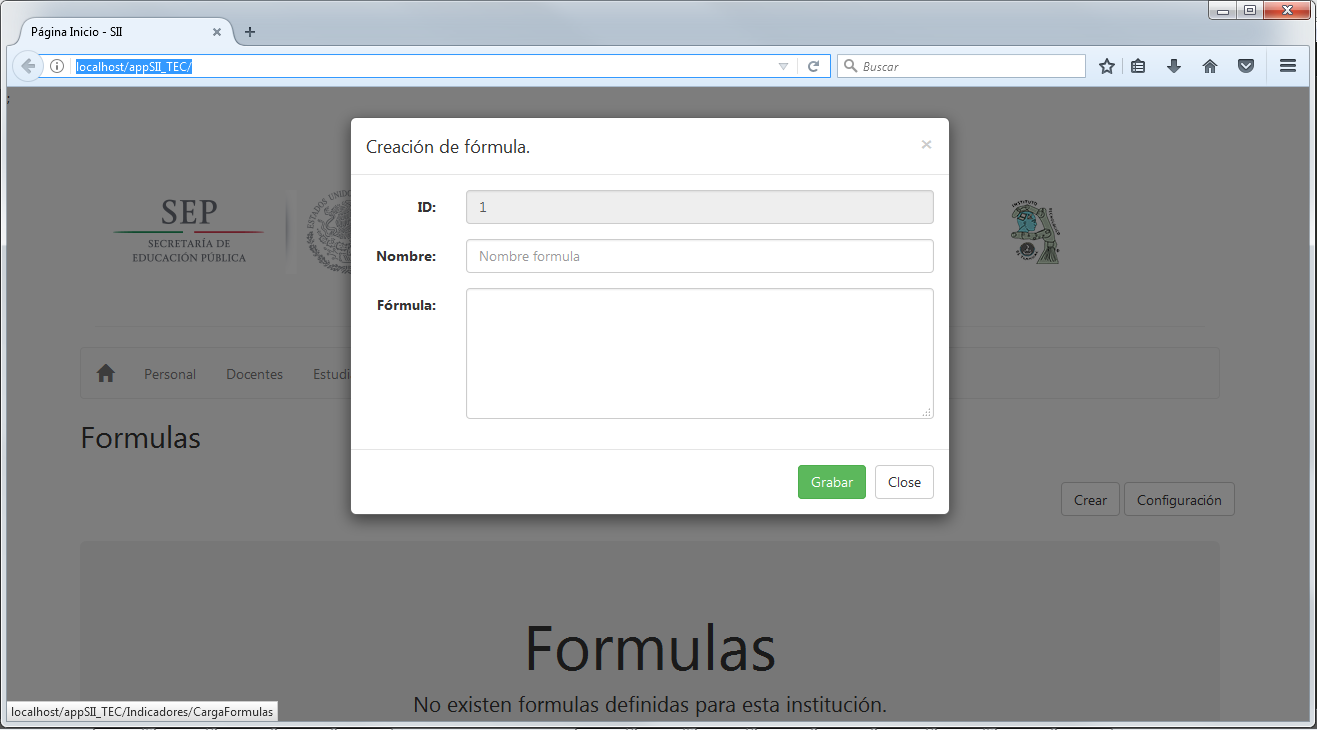
\includegraphics[width=16cm, height=9.5cm]{figuras/FormulasCrear}
		        \caption{Ventana emergente para creaci\'on de f\'ormulas.}
		        \label{fig_FormulasCrear}
		    \end{figure}
			
			Los datos que se solicitan para la creaci\'on de una f\'ormula son los siguientes:
			\begin{enumerate}[1.]
				\item \textbf{ID:} N\'umero identificador, este se genera de manera autom\'atica, es por esto que se muestra deshabilitado.
				\item \textbf{Nombre:} Campo para especificar el nombre con el que se identificar\'a la f\'ormula.
				\item \textbf{f\'ormula:} Campo para definir la f\'ormula.
			\end{enumerate}

			Cuando uno de estos datos no se ingresa correctamente, se muestra un mensaje de error tal como se muestra en la figura \ref{fig_FormulaValida}.\\

			\begin{figure}[]
		        \centering
		        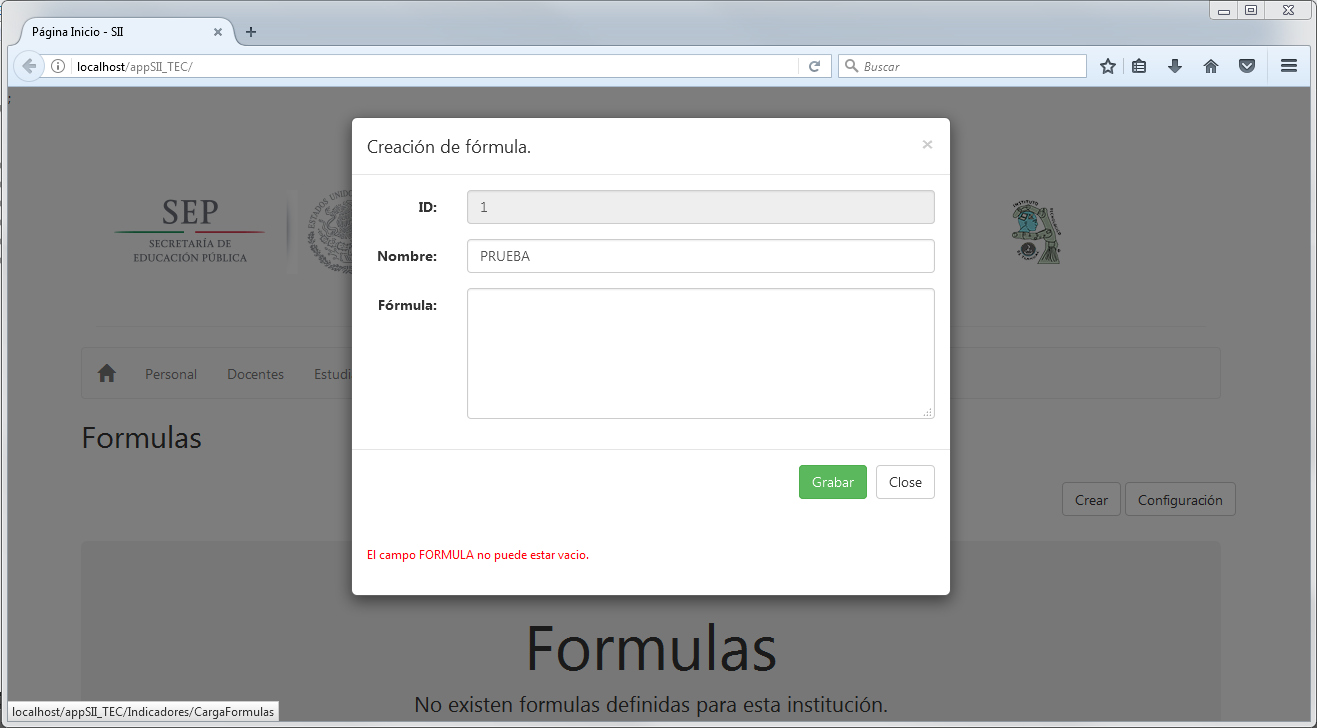
\includegraphics[width=16cm, height=9.5cm]{figuras/FormulaValida}
		        \caption{Mensaaje de validaci\'on f\'ormulas.}
		        \label{fig_FormulaValida}
		    \end{figure}

		    Al momento de ingresar los datos correctamente, el sistema graba el registro en la base de datos y manda un mensaje indicando que el proceso se realiz\'o correctamente, esto se muestra en la figura \ref{img_FormulasGraba}.\\

		    \begin{figure}[]
		        \centering
		        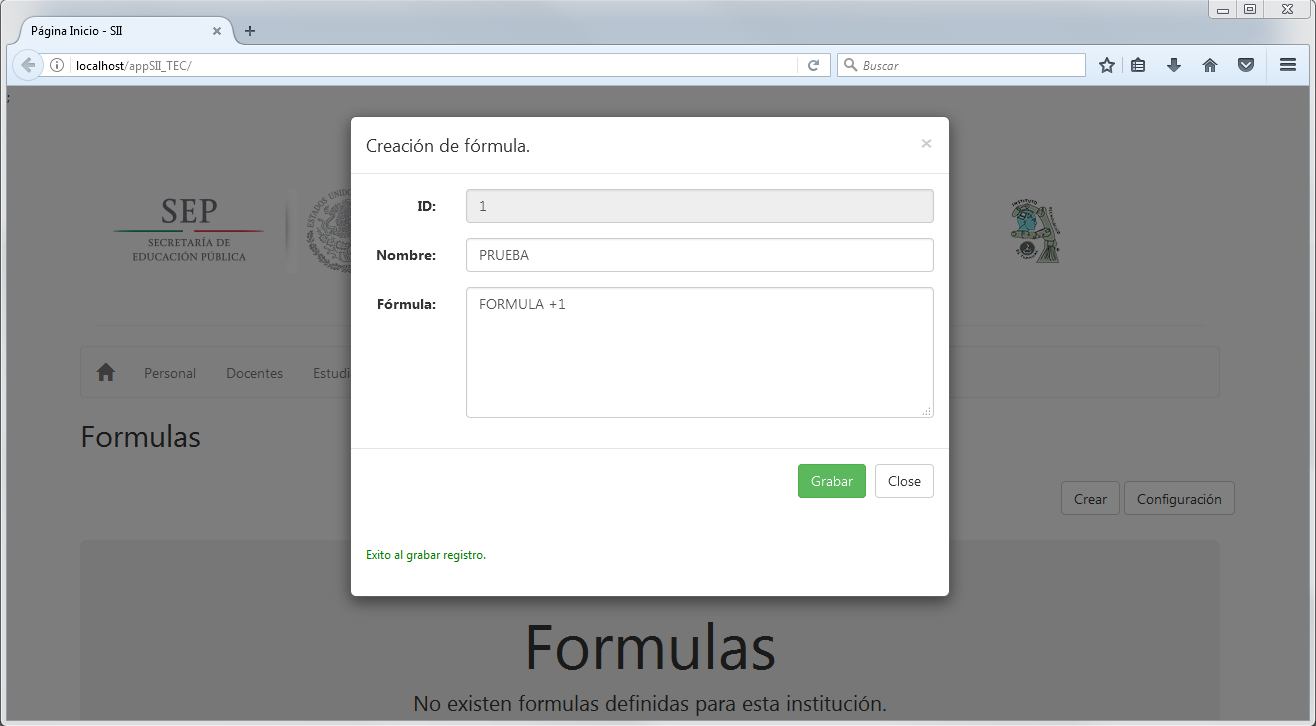
\includegraphics[width=16cm, height=9.5cm]{figuras/FormulasGraba}
		        \caption{Mensaaje de grabaci\'on satisfactoria de f\'ormula.}
		        \label{img_FormulasGraba}
		    \end{figure}

		    Una vez que existen f\'ormulas registrados en la base de datos, estos se muestran en una tabla, la cual tendr\'a dos acciones espec\'ificas por f\'ormula, una es actualizar y la otra es eliminar. Esta tabla de f\'ormula se muestra en la figura \ref{fig_FormulasTabla}.\\

		    \begin{figure}[]
		        \centering
		        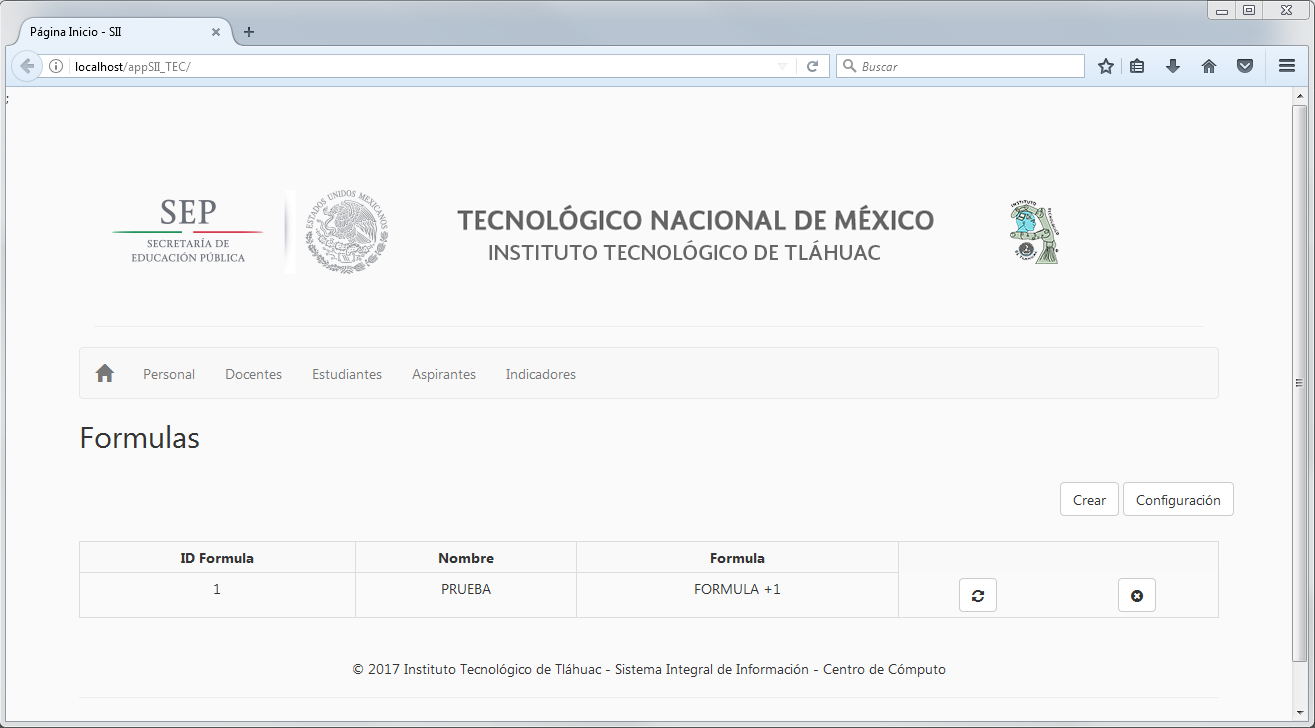
\includegraphics[width=16cm, height=9.5cm]{figuras/FormulasTabla}
		        \caption{Listado de f\'ormulas.}
		        \label{fig_FormulasTabla}
		    \end{figure}
			
			\subsection{Actualizaci\'on de f\'ormulas}

			Para la actualizaci\'on de f\'ormulas se muestra la misma ventana emergente que se usa para crear una, pero en este caso se visualizan los datos de la f\'ormula que se seleccion\'o. En este caso se muestra la ventana emergente en la que se quiere actualizar la f\'ormula de PRUEBA, esta ventana se muestra en la figura \ref{fig_FormulasActualiza}.

			\begin{figure}[]
		        \centering
		        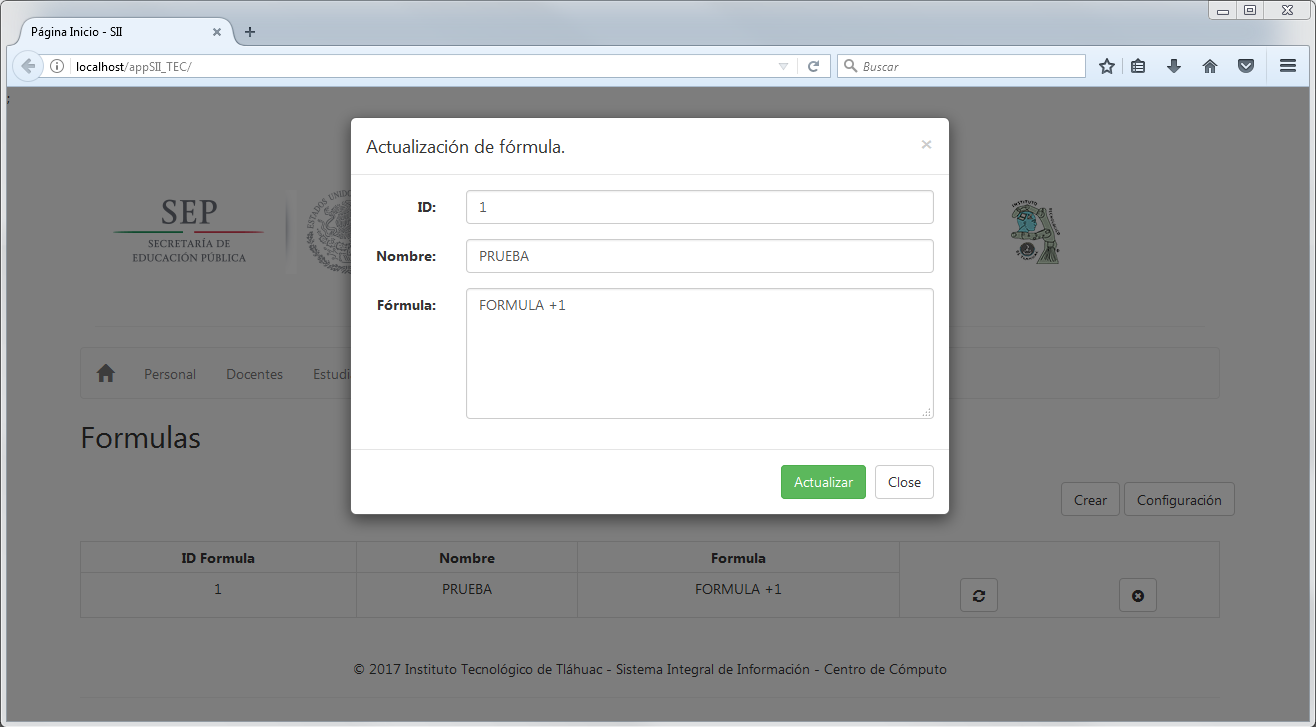
\includegraphics[width=16cm, height=9.5cm]{figuras/FormulasActualiza}
		        \caption{Ventana emergente de actualizaci\'on de f\'ormula.}
		        \label{fig_FormulasActualiza}
		    \end{figure}

		    \subsection{Baja de f\'ormulas}

		    Como \'ultima prueba se muestra en la figura \ref{fig_FormulasElimina} la ventana emergente mostrada al momento de querer eliminar una f\'ormula, el sistema pregunta al usuario si esta seguro de eliminar este registr\'o.\\

		    \begin{figure}[]
		        \centering
		        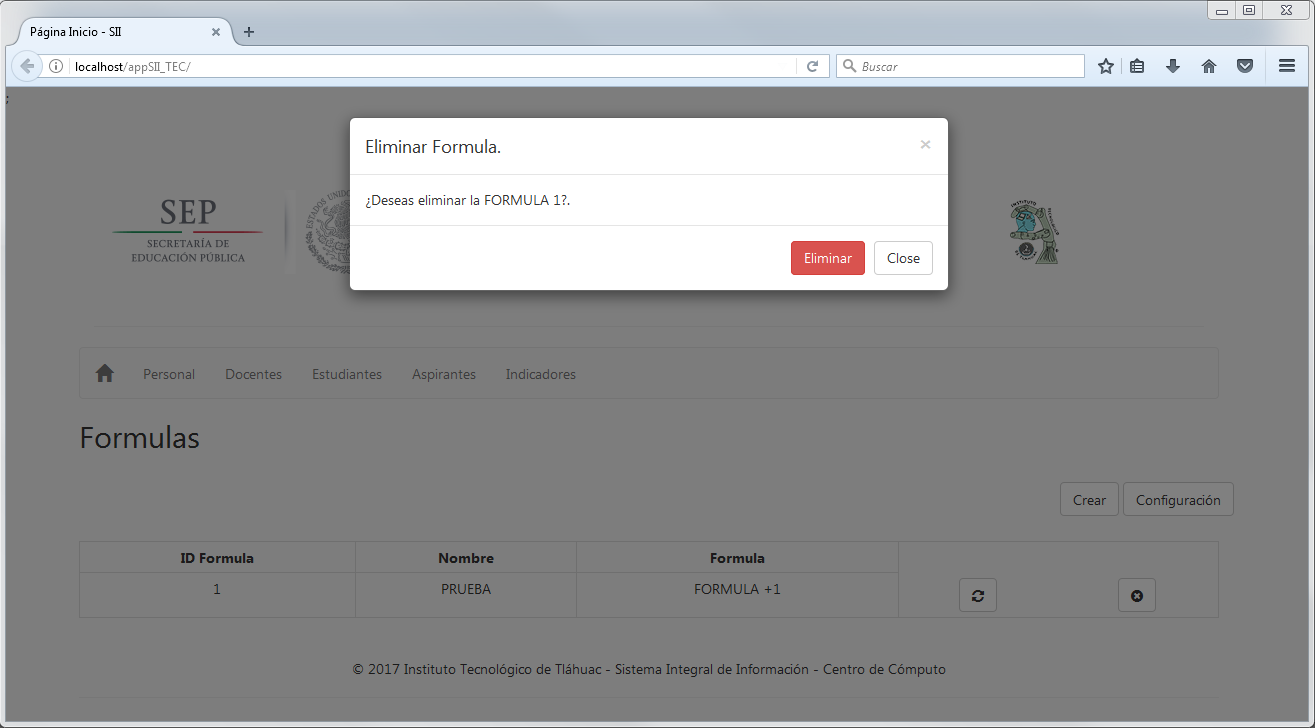
\includegraphics[width=16cm, height=9.5cm]{figuras/FormulasElimina}
		        \caption{Mensaje de advertencia al eliminar f\'ormula.}
		        \label{fig_FormulasElimina}
		    \end{figure}








		\section{Pruebas y resultados de m\'odulo Colecciones.}

			Para ingresar al m\'odulo de configuraci\'on de colecciones, es necesario dar click en el bot\'on Configuraci\'on $\rightarrow$ Colecciones, lo cual nos mostrara la ventana ilustrada en la figura \ref{fig_Colecciones}.\\


			\begin{figure}[]
		        \centering
		        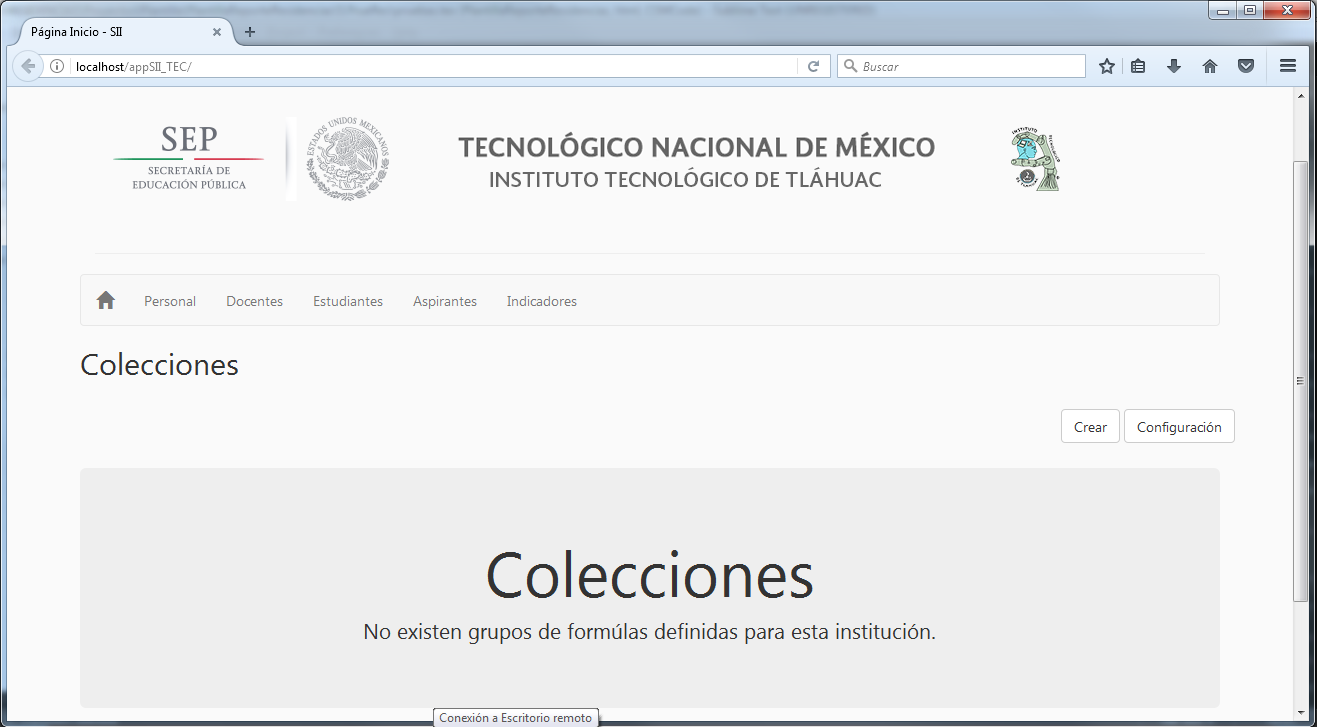
\includegraphics[width=16cm, height=9.5cm]{figuras/Colecciones}
		        \caption{Pantalla principal de colecciones.}
		        \label{fig_Colecciones}
		    \end{figure}
			
			El m\'odulo de colecciones cuenta con las siguientes funciones para validar:
			\begin{itemize}
				\item Alta de colecciones.
				\item Actualizaci\'on de colecciones.
				\item Baja de colecciones.
				\item Detalle de colecciones.
			\end{itemize}

			Estas acciones se muestran a continuaci\'on:

			\subsection{Alta de colecci\'on}

			Para crear una colecci\'on, se tiene que dar click en el bot\'on crear del m\'odulo de configuraci\'on de colecciones, mostrando con esto la ventana emergente  que se puede ver en la figura \ref{fig_ColeccionesCrear}.\\

			\begin{figure}[]
		        \centering
		        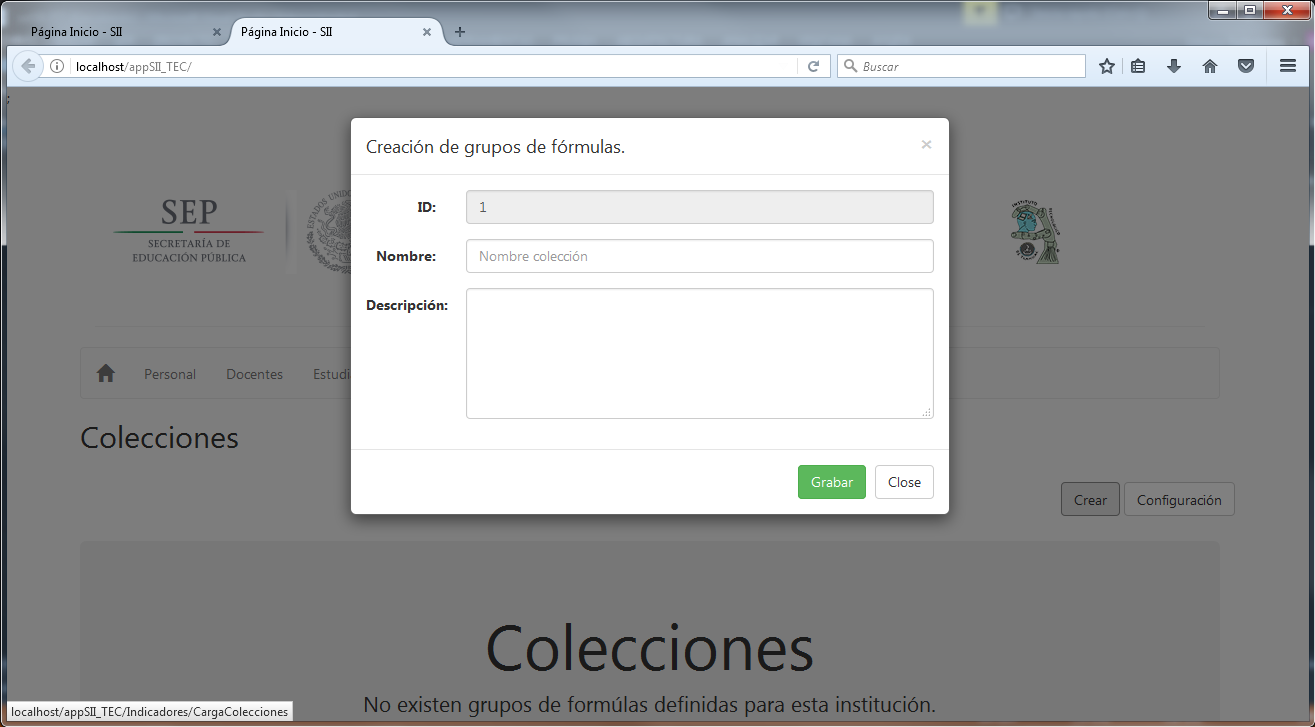
\includegraphics[width=16cm, height=9.5cm]{figuras/ColeccionesCrear}
		        \caption{Ventana emergente para creaci\'on de colecciones.}
		        \label{fig_ColeccionesCrear}
		    \end{figure}
			
			Los datos que se solicitan para la creaci\'on de una colecci\'on son los siguientes:
			\begin{enumerate}[1.]
				\item \textbf{ID:} N\'umero identificador, este se genera de manera autom\'atica, es por esto que se muestra deshabilitado.
				\item \textbf{Nombre:} Campo para especificar el nombre con el que se identificar\'a la f\'ormula.
				\item \textbf{Descripci\'o:} Campo para almacenar una breve descripci\'on de la colecci\'on.
			\end{enumerate}

			Cuando uno de estos datos no se ingresa correctamente, se muestra un mensaje de error tal como se muestra en la figura \ref{fig_ColeccionesValida}.\\

			\begin{figure}[]
		        \centering
		        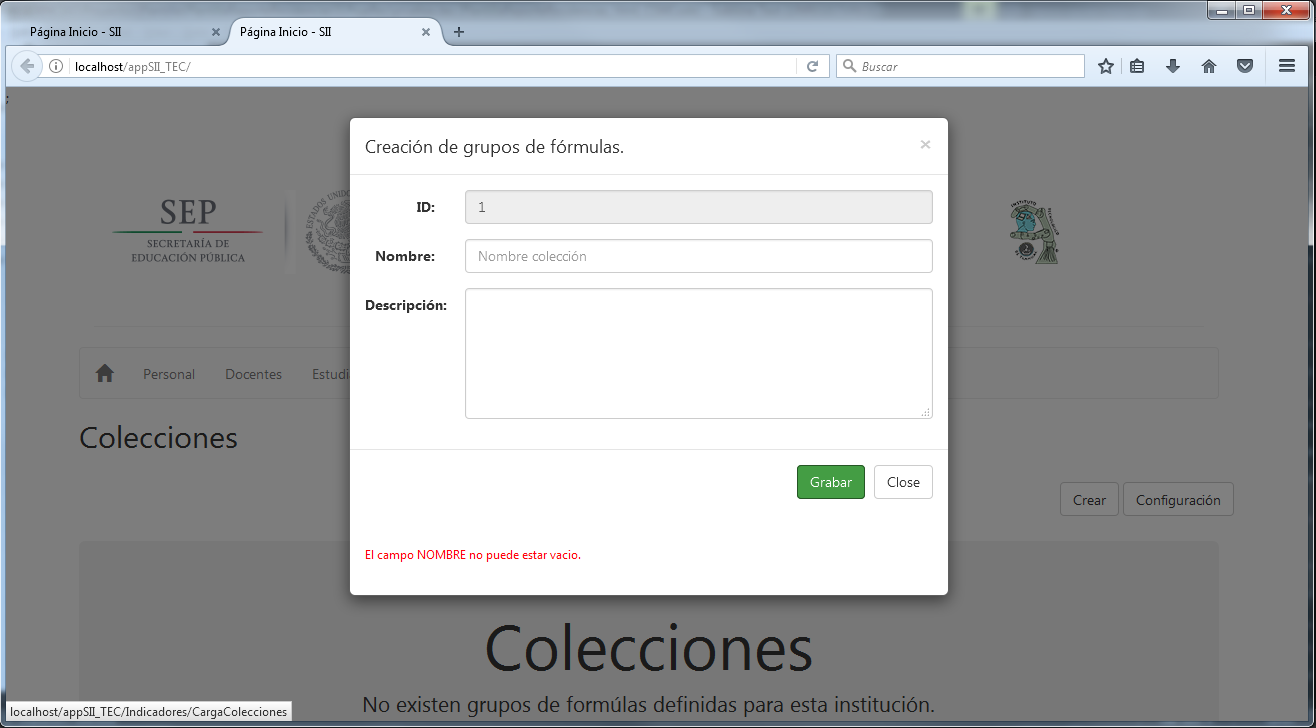
\includegraphics[width=16cm, height=9.5cm]{figuras/ColeccionesValida}
		        \caption{Mensaaje de validaci\'on colecciones.}
		        \label{fig_ColeccionesValida}
		    \end{figure}

		    Al momento de ingresar los datos correctamente, el sistema graba el registro en la base de datos y manda un mensaje indicando que el proceso se realiz\'o correctamente, esto se muestra en la figura \ref{img_ColeccionesGraba}.\\

		    \begin{figure}[]
		        \centering
		        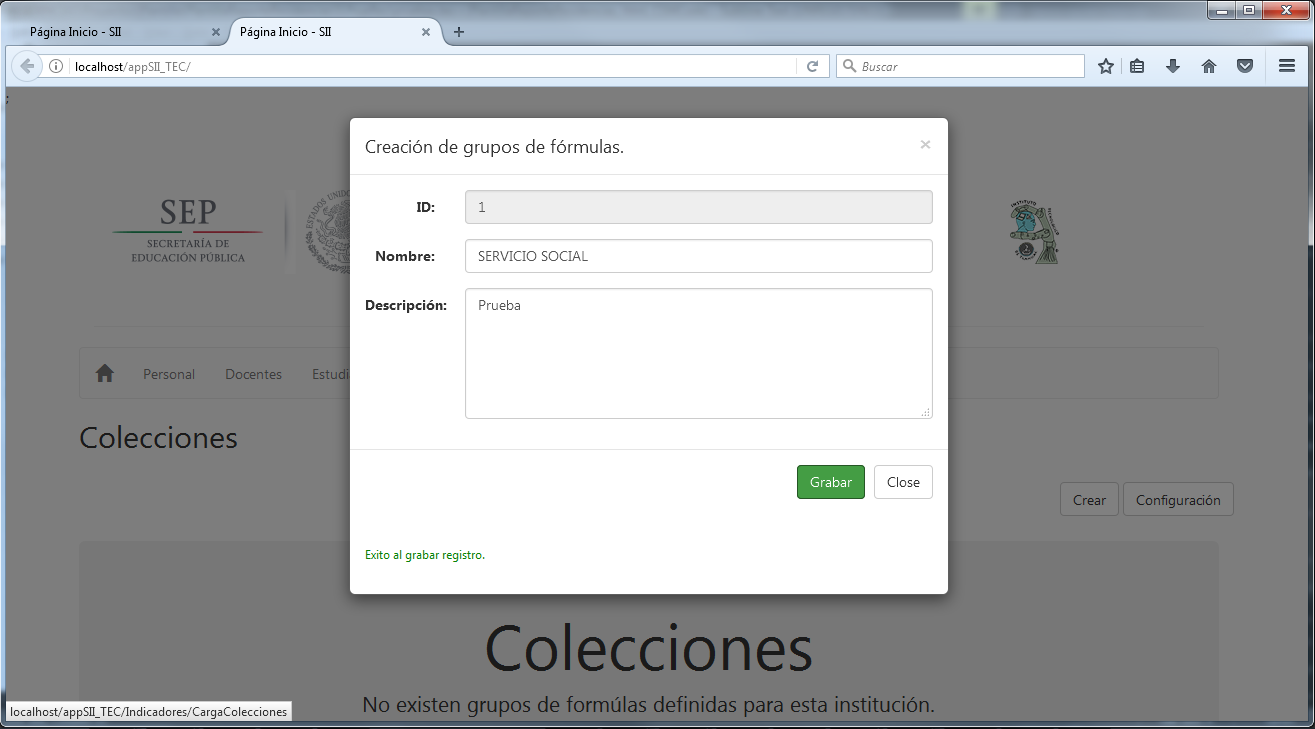
\includegraphics[width=16cm, height=9.5cm]{figuras/ColeccionesGraba}
		        \caption{Mensaaje de grabaci\'on satisfactoria de colecci\'on.}
		        \label{img_ColeccionesGraba}
		    \end{figure}

		    Una vez que existen colecciones registrados en la base de datos, estos se muestran en una tabla, la cual tendr\'a dos acciones espec\'ificas por colecci\'on, una es actualizar, la otra es mostrar el detalle de la colecci\'on y por ultimo eliminar. Esta tabla de f\'ormula se muestra en la figura \ref{fig_ColeccionesTabla}.\\

		    \begin{figure}[]
		        \centering
		        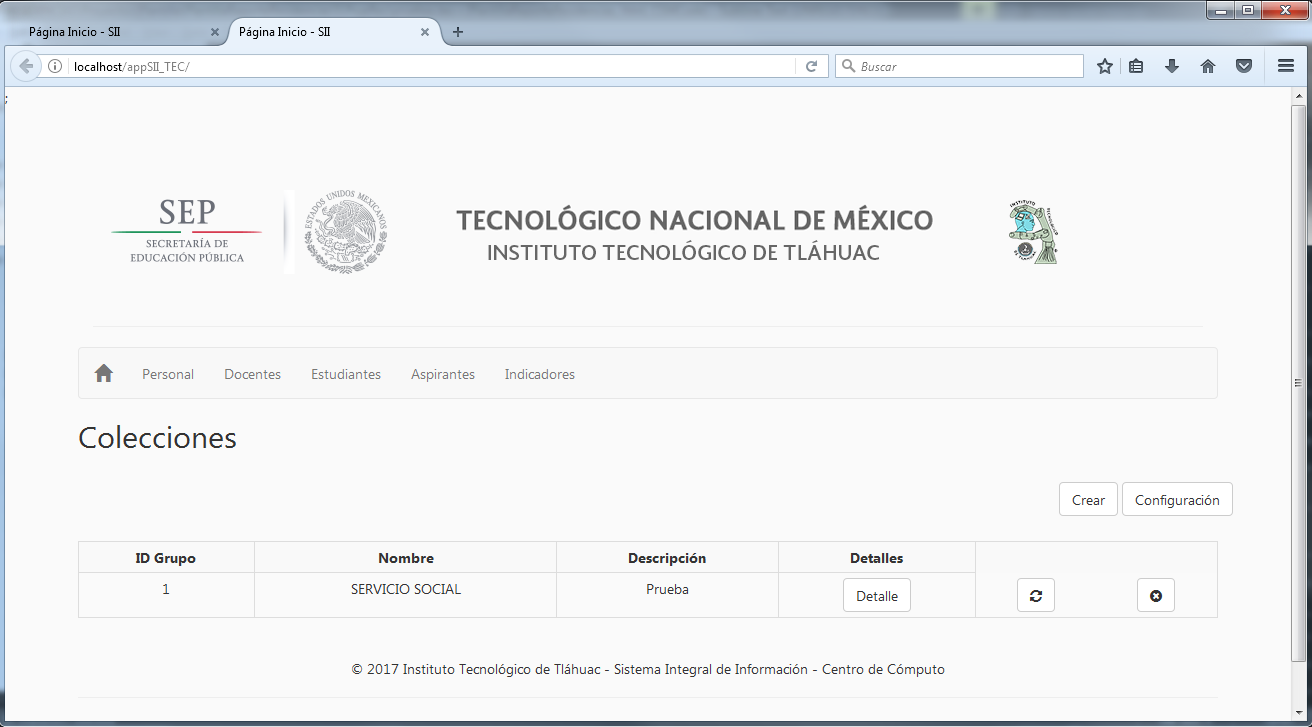
\includegraphics[width=16cm, height=9.5cm]{figuras/ColeccionesTabla}
		        \caption{Listado de colecciones.}
		        \label{fig_ColeccionesTabla}
		    \end{figure}
			
			\subsection{Actualizaci\'on de colecciones}

			Para la actualizaci\'on de colecciones se muestra la misma ventana emergente que se usa para crear una, pero en este caso se visualizan los datos de la colecci\'on que se seleccion\'o. En este caso se muestra la ventana emergente en la que se quiere actualizar la colecci\'on de SERVICIO SOCIAL, esta ventana se muestra en la figura \ref{fig_ColeccionesActualiza}.

			\begin{figure}[]
		        \centering
		        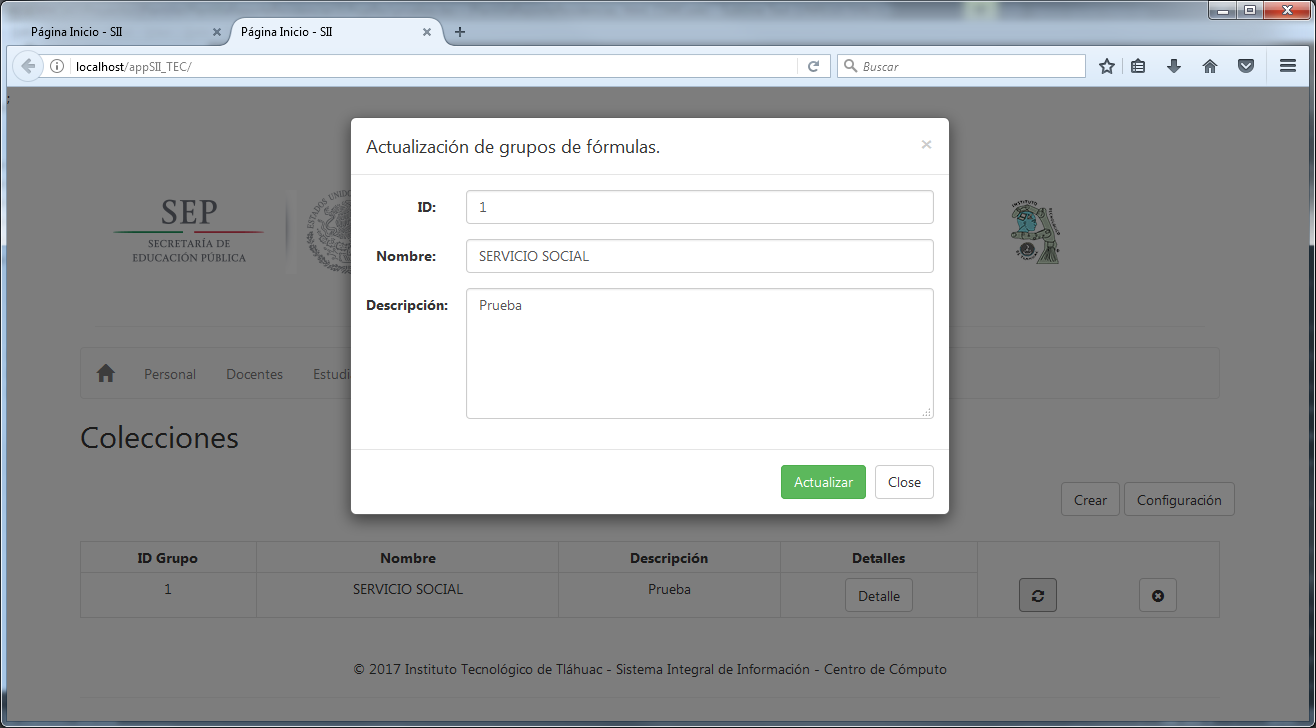
\includegraphics[width=16cm, height=9.5cm]{figuras/ColeccionesActualiza}
		        \caption{Ventana emergente de actualizaci\'on de colecciones.}
		        \label{fig_ColeccionesActualiza}
		    \end{figure}

		    \subsection{Baja de colecci\'on}

		    Como \'ultima prueba se muestra en la figura \ref{fig_ColeccionesElimina} la ventana emergente mostrada al momento de querer eliminar una colecci\'on, el sistema pregunta al usuario si esta seguro de eliminar este registr\'o.\\

		    \begin{figure}[]
		        \centering
		        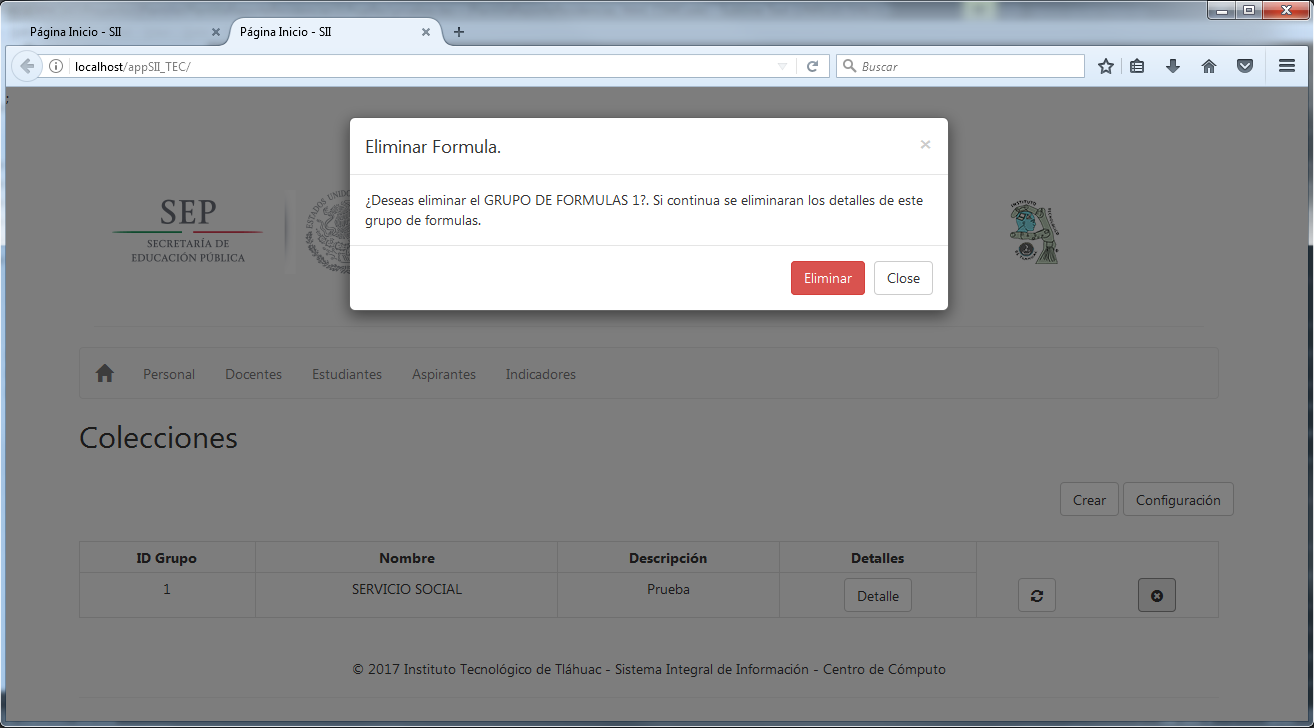
\includegraphics[width=16cm, height=9.5cm]{figuras/ColeccionesElimina}
		        \caption{Mensaje de advertencia al eliminar colecci\'on.}
		        \label{fig_ColeccionesElimina}
		    \end{figure}

		    \subsection{Detalle de colecciones}

		    Esta funcionalidad es para mostrar las f\'ormulas que est\'an contenidas dentro de esta colecci\'on, para esto al dar click en el bot\'on Detalle que se encuentra en cada fila de las colecciones. Al ejecutar esta funci\'on se mostrara una nueva pantalla como se muestra en la figura 

		    \begin{figure}[]
		        \centering
		        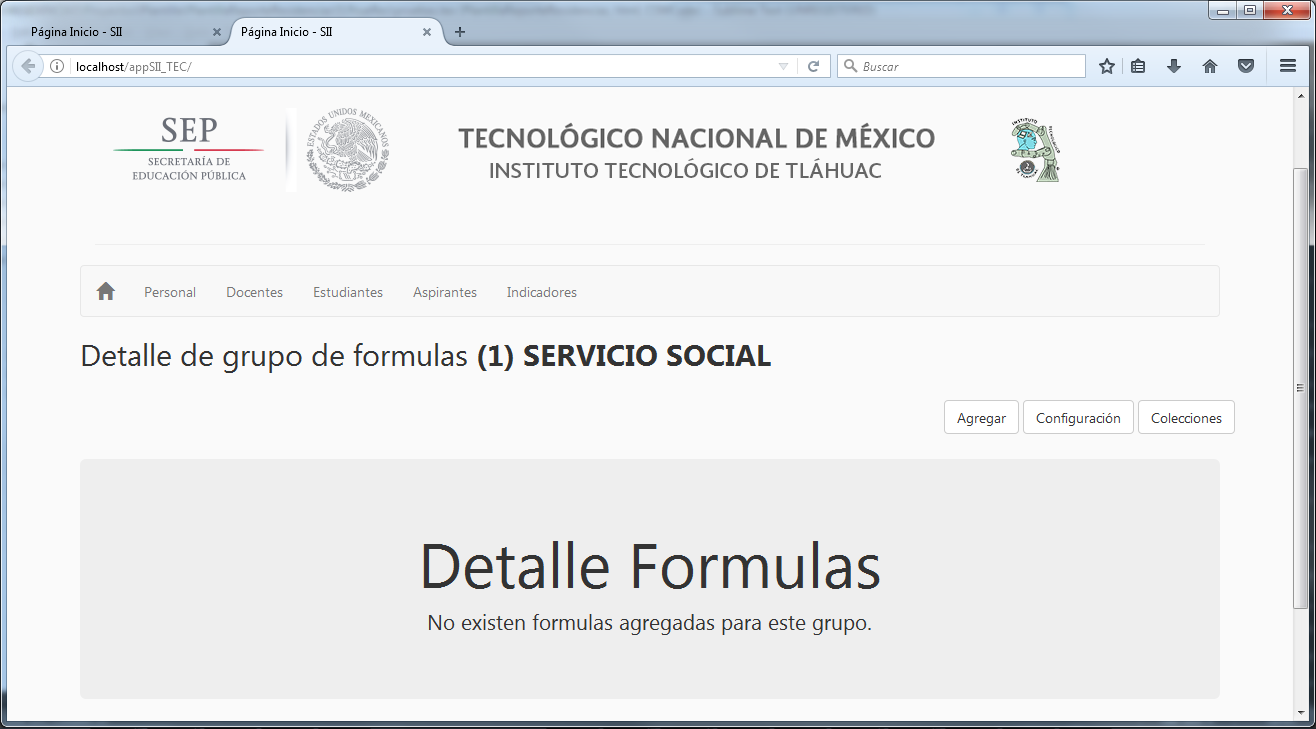
\includegraphics[width=16cm, height=9.5cm]{figuras/ColeccionesDetalle}
		        \caption{Pantalla de inicio del detalle de colecciones.}
		        \label{fig_ColeccionesDetalle}
		    \end{figure}

		    Las acciones que se pueden realizar dentro de este m\'odulo son:
		    \begin{itemize}
		    	\item Agregar formulas a colecci\'on.
		    	\item Quitar f\'ormulas de colecci\'on.
		    \end{itemize}

		    \subsubsection{Agregar formulas a colecci\'on}

		    	Esta funcionalidad se ejecuta al momento de presionar el bot\'on agregar, el cual abre una ventana emergente que contiene la lista de f\'ormulas disponibles para ser agregadas a la colecci\'on. Estas se describen en la figura \ref{fig_ColeccionesDetalleAgregar} la cual muestra c\'omo se pueden seleccionar m\'ultiples f\'ormulas para ser agregadas.\\

		    	\begin{figure}[]
			        \centering
			        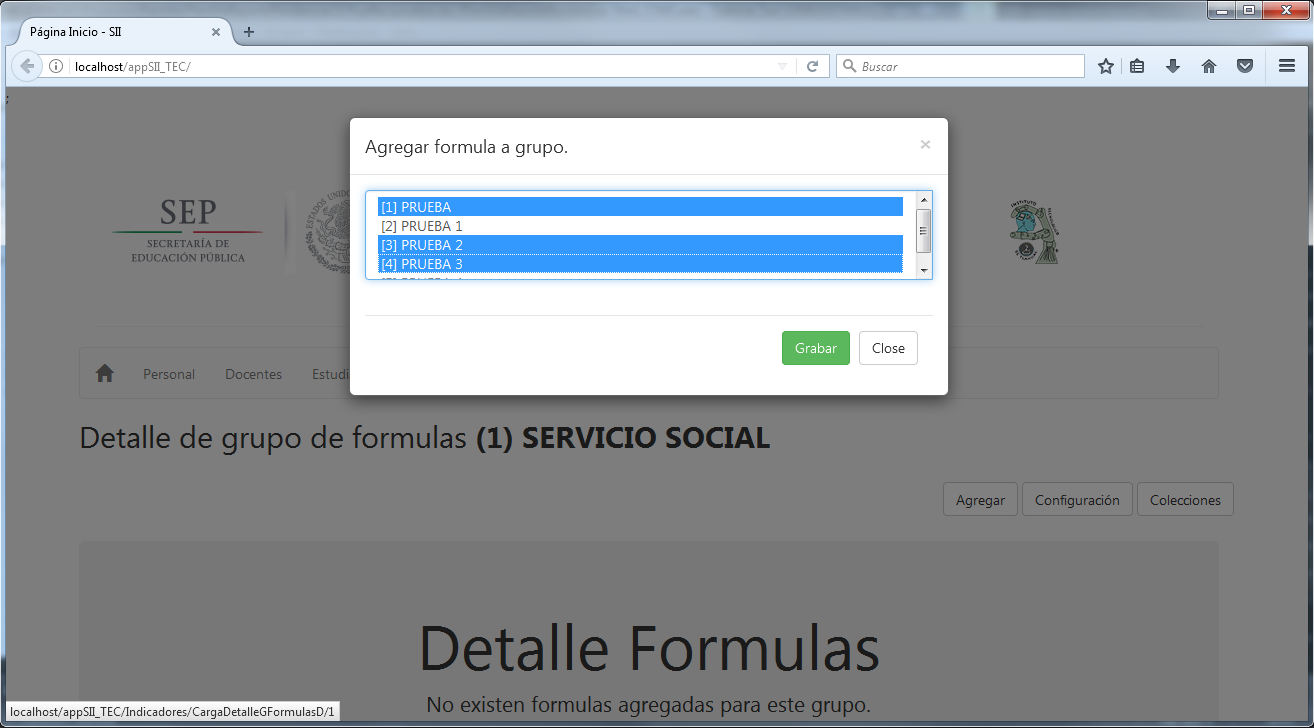
\includegraphics[width=16cm, height=9.5cm]{figuras/ColeccionesDetalleAgregar}
			        \caption{Ventana emergente para agregar formulas a colecci\'on.}
			        \label{fig_ColeccionesDetalleAgregar}
			    \end{figure}

			    Al dar click en Grabar, el sistema mostrara un mensaje indicando si el proceso se ejecut\'o de manera correcta o no como se muestra en la figura \ref{fig_ColeccionesDetalleGrabar}. El listado de las f\'ormulas que pertenecen a la coleccion se visualiza en la figura \ref{fig_ColeccionesDetalleTabla}.

			    \begin{figure}[]
			        \centering
			        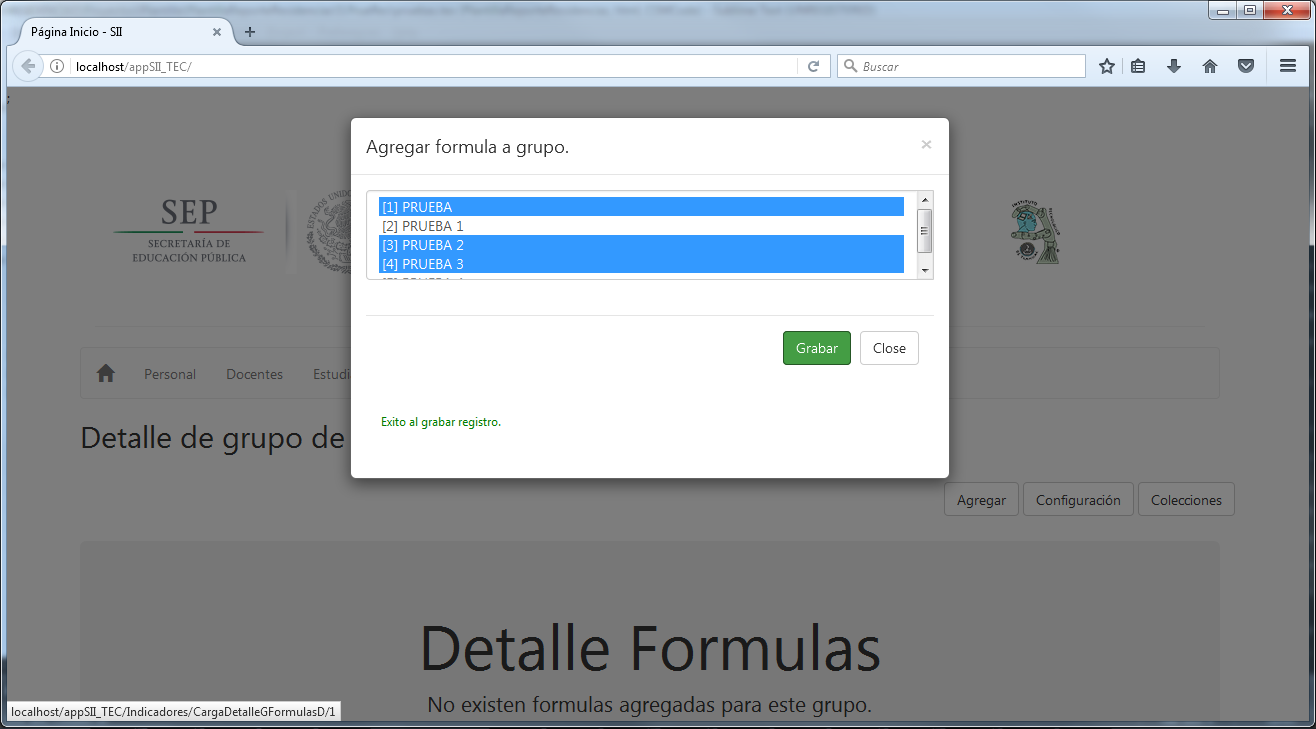
\includegraphics[width=16cm, height=9.5cm]{figuras/ColeccionesDetalleGrabar}
			        \caption{Mensaje de grabaci\'on satisfactoria de formulas en colecci\'on.}
			        \label{fig_ColeccionesDetalleGrabar}
			    \end{figure}

			    \begin{figure}[]
			        \centering
			        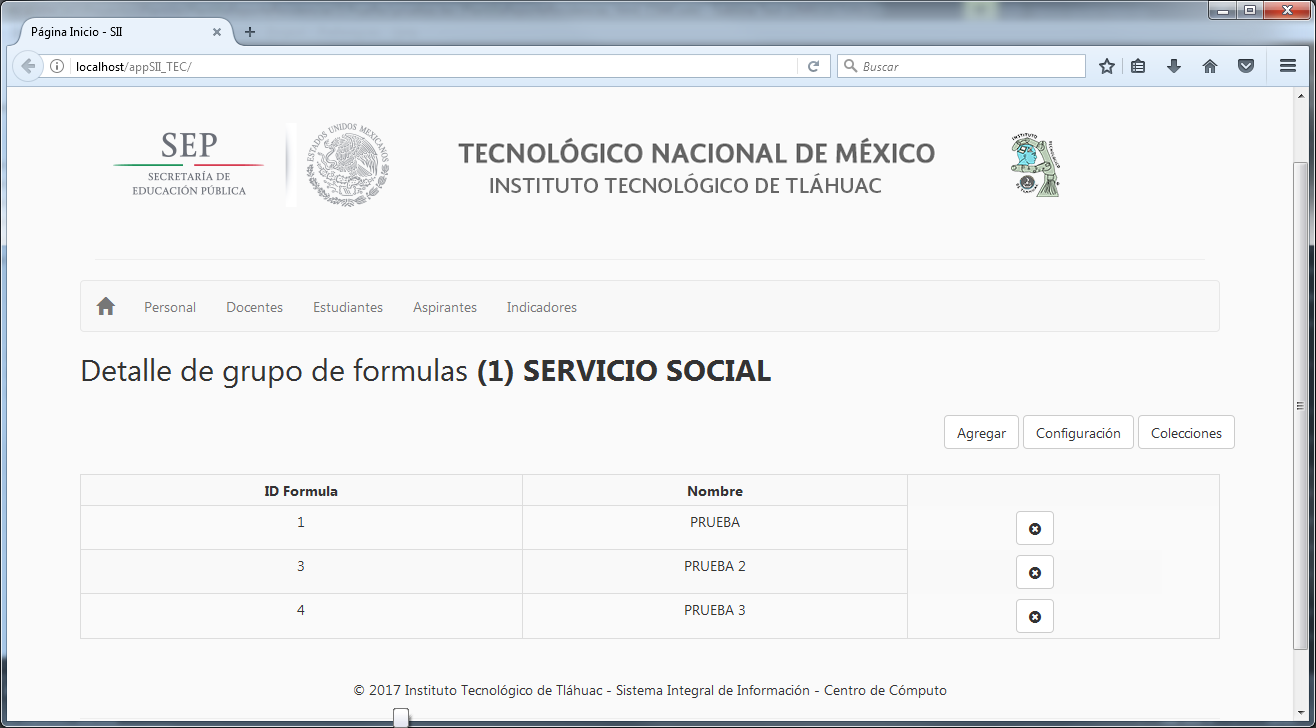
\includegraphics[width=16cm, height=9.5cm]{figuras/ColeccionesDetalleTabla}
			        \caption{Listado de f\'ormulas en colecci\'on.}
			        \label{fig_ColeccionesDetalleTabla}
			    \end{figure}

			\subsubsection{Quitar f\'ormulas de colecci\'on}

				En esta permite quitar una f\'ormula de la colecci\'on. Esta funci\'on se ejecuta cuando presionamos el bot\'on Eliminar que se encuentra en cada registro. Al ejecutar dicha funcionalidad se preguntara al usuario si desea continuar como se muestra en la figura \ref{fig_ColeccionesDetalleEliminar}.

				\begin{figure}[]
			        \centering
			        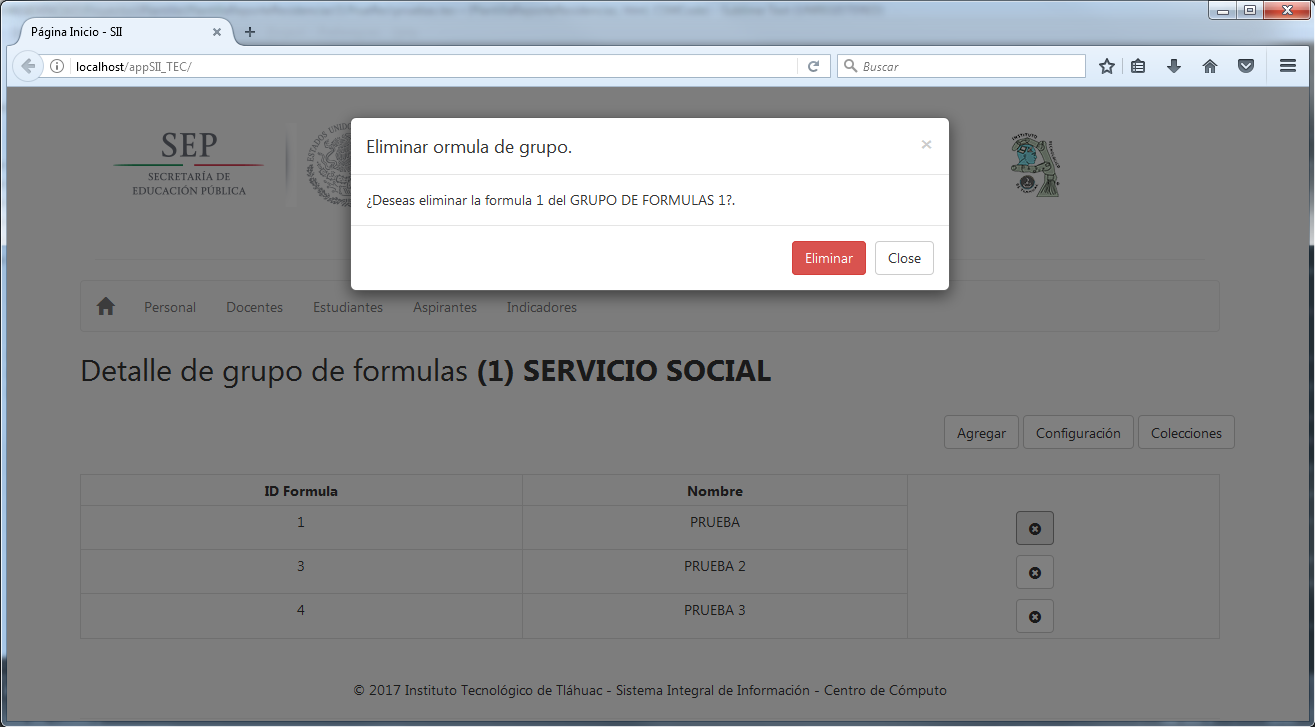
\includegraphics[width=16cm, height=9.5cm]{figuras/ColeccionesDetalleEliminar}
			        \caption{Mensaje de advertencia al eliminar una formula de colecci\'on.}
			        \label{fig_ColeccionesDetalleEliminar}
			    \end{figure}














		\section{Pruebas y resultados de m\'odulo Proceso.}
			   

			Para ingresar al m\'odulo de proceso de indicadores, es necesario dar click en el bot\'on Proceso que se encuentra en la pagina principal, lo cual nos mostrara la ventana ilustrada en la figura \ref{fig_Formulas}.


			\begin{figure}[H]
		        \centering
		        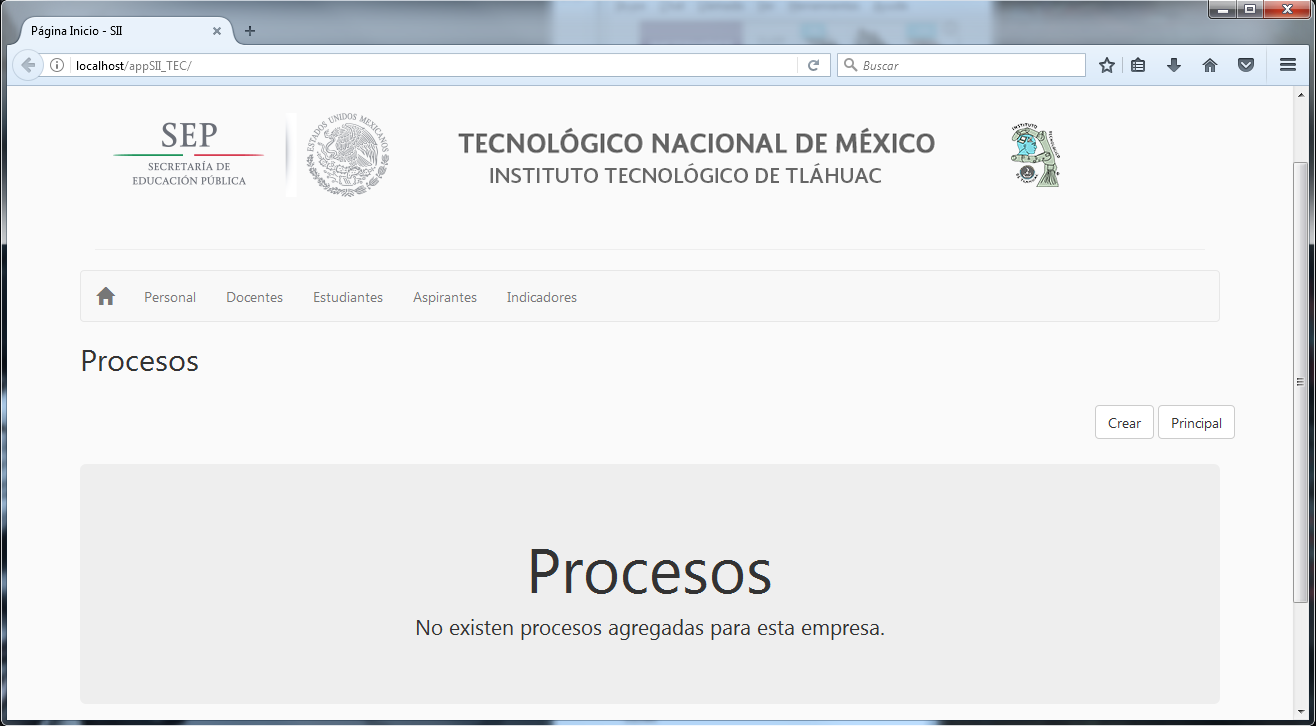
\includegraphics[width=16cm, height=9.5cm]{figuras/Procesos}
		        \caption{Pantalla principal de procesos.}
		        \label{fig_Procesos}
		    \end{figure}
			
			El m\'odulo de procesos cuenta con las siguientes funciones para validar:
			\begin{itemize}
				\item Alta de periodos.
				\item Actualizaci\'on de periodos.
				\item Baja de periodos.
				\item Proceso de periodos.
				\item Visualizaci\'on del detalle de procesos.
			\end{itemize}

			Estas acciones se muestran a continuaci\'on:

			\subsection{Alta de Procesos}

			Para crear una periodo de indicadores, se tiene que dar click en el bot\'on crear del m\'odulo de configuraci\'on de periodos, mostrando con esto la ventana emergente  que se puede ver en la figura \ref{fig_ProcesoCrear}.\\

			\begin{figure}[]
		        \centering
		        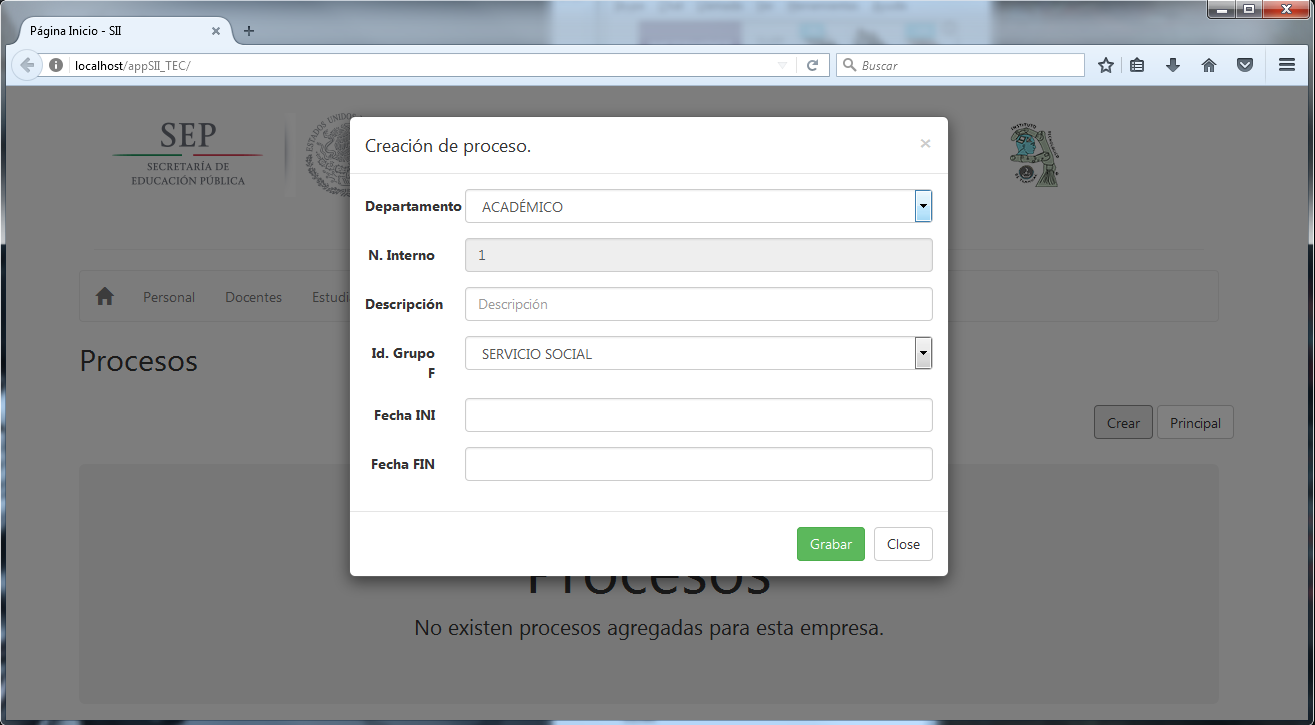
\includegraphics[width=16cm, height=9.5cm]{figuras/ProcesoCrear}
		        \caption{Ventana emergente para creaci\'on de periodos de indicadores.}
		        \label{fig_ProcesoCrear}
		    \end{figure}
			
			Los datos que se solicitan para la creaci\'on de un periodo de indicadores son los siguientes:
			\begin{enumerate}[1.]
				\item \textbf{Departamento:} N\'umero de departament al que pertenece el periodo.
				\item \textbf{N\'umero interno:} Valor identificador del periodo de indicadores.
				\item \textbf{Descripci\'on:} Campo para dar detalle de lo que se est\'a procesando en el periodo.
				\item \textbf{ID Colecci\'on de f\'ormulas:} N\'umero de colecci\'on de f\'ormulas a procesar.
				\item \textbf{Fecha inicial:} Fecha en la que el periodo inicia.
				\item \textbf{Fecha final:} Fecha en la que el periodo termina.
			\end{enumerate}

			Cuando uno de estos datos no se ingresa correctamente, se muestra un mensaje de error tal como se muestra en la figura \ref{fig_ProcesoValida}.\\

			\begin{figure}[]
		        \centering
		        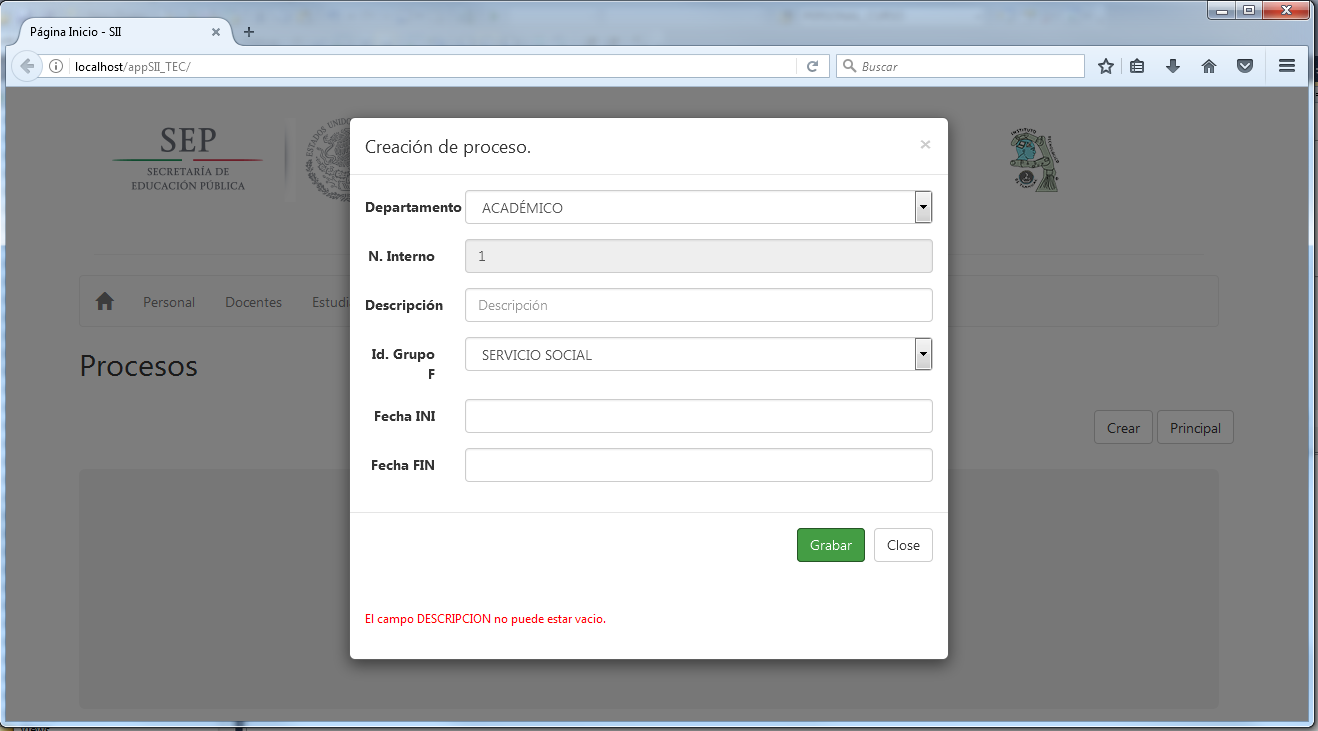
\includegraphics[width=16cm, height=9.5cm]{figuras/ProcesoValida}
		        \caption{Mensaaje de validaci\'on en proceso de indicadores.}
		        \label{fig_ProcesoValida}
		    \end{figure}

		    Al momento de ingresar los datos correctamente, el sistema graba el registro en la base de datos y manda un mensaje indicando que el proceso se realiz\'o correctamente, esto se muestra en la figura \ref{img_ProcesoGraba}.\\

		    \begin{figure}[]
		        \centering
		        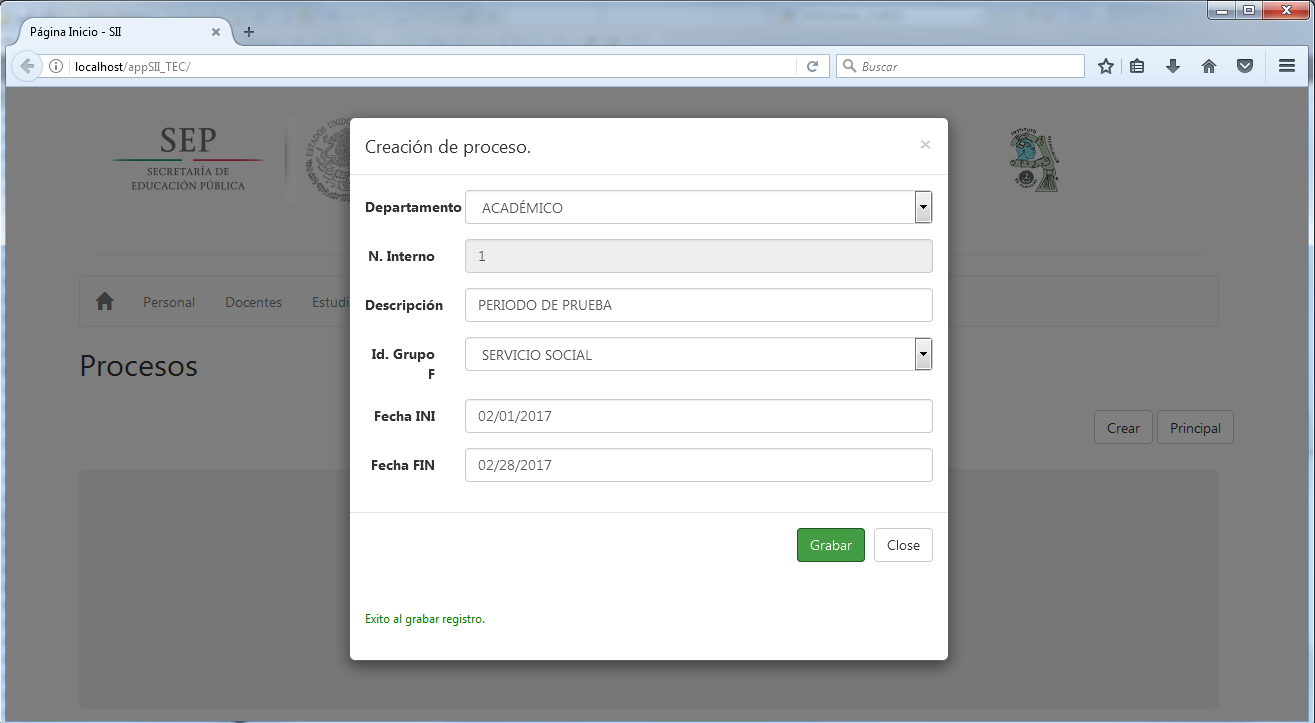
\includegraphics[width=16cm, height=9.5cm]{figuras/ProcesoGraba}
		        \caption{Mensaaje de grabaci\'on satisfactoria de procesos de indicadores.}
		        \label{img_ProcesoGraba}
		    \end{figure}

		    Una vez que existen procesos registrados en la base de datos, estos se muestran en una tabla, la cual tendr\'a acciones espec\'ificas por proceso, las acciones por proceso son actualizar, eliminar, procesar y mostrar detalle de proceso. Esta tabla de procesos se muestra en la figura \ref{fig_ProcesoTabla}.\\

		    \begin{figure}[]
		        \centering
		        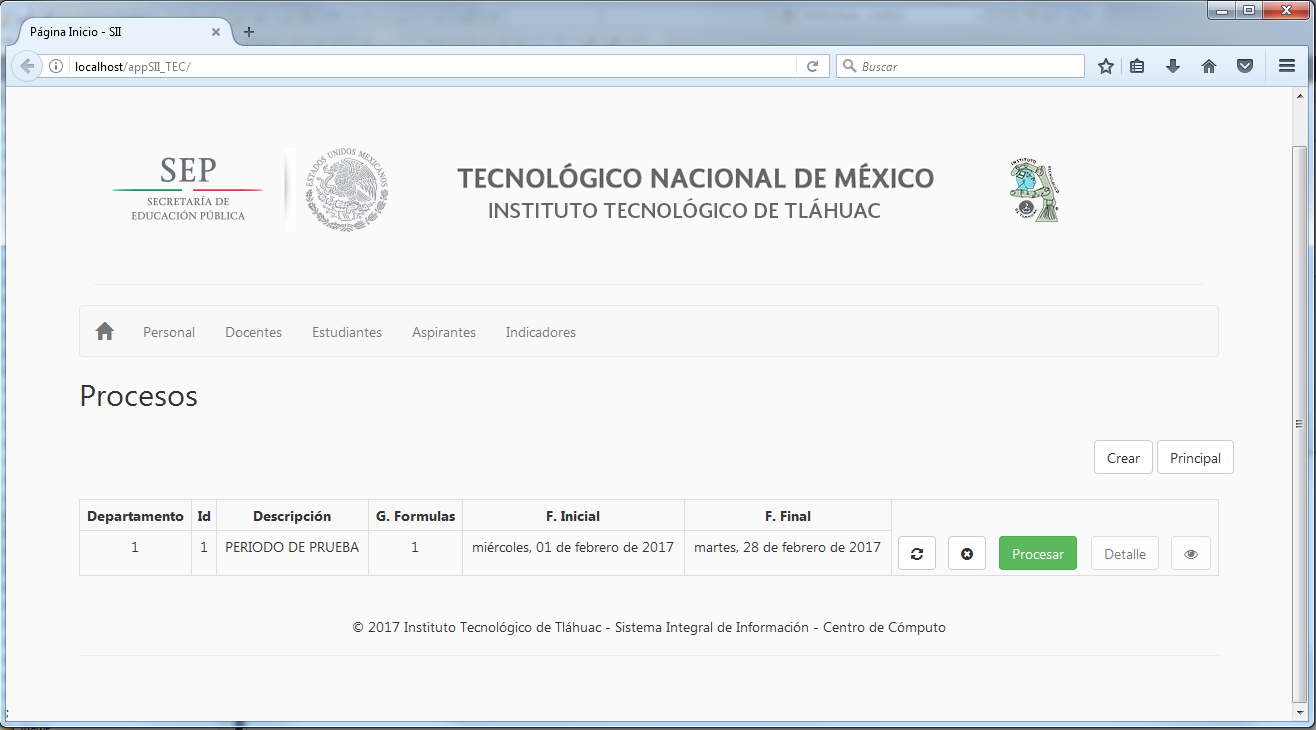
\includegraphics[width=16cm, height=9.5cm]{figuras/ProcesoTabla}
		        \caption{Listado de procesos.}
		        \label{fig_ProcesoTabla}
		    \end{figure}
			
			\subsection{Actualizaci\'on de procesos}

			Para la actualizaci\'on de procesos se muestra la misma ventana emergente que se usa para crear uno, pero en este caso se visualizan los datos del proceso que se seleccion\'o. En este caso se muestra la ventana emergente en la que se quiere actualizar el proceso con el nombre PERIODO DE PRUEBA, esta ventana se muestra en la figura \ref{fig_ProcesoActualiza}.

			\begin{figure}[]
		        \centering
		        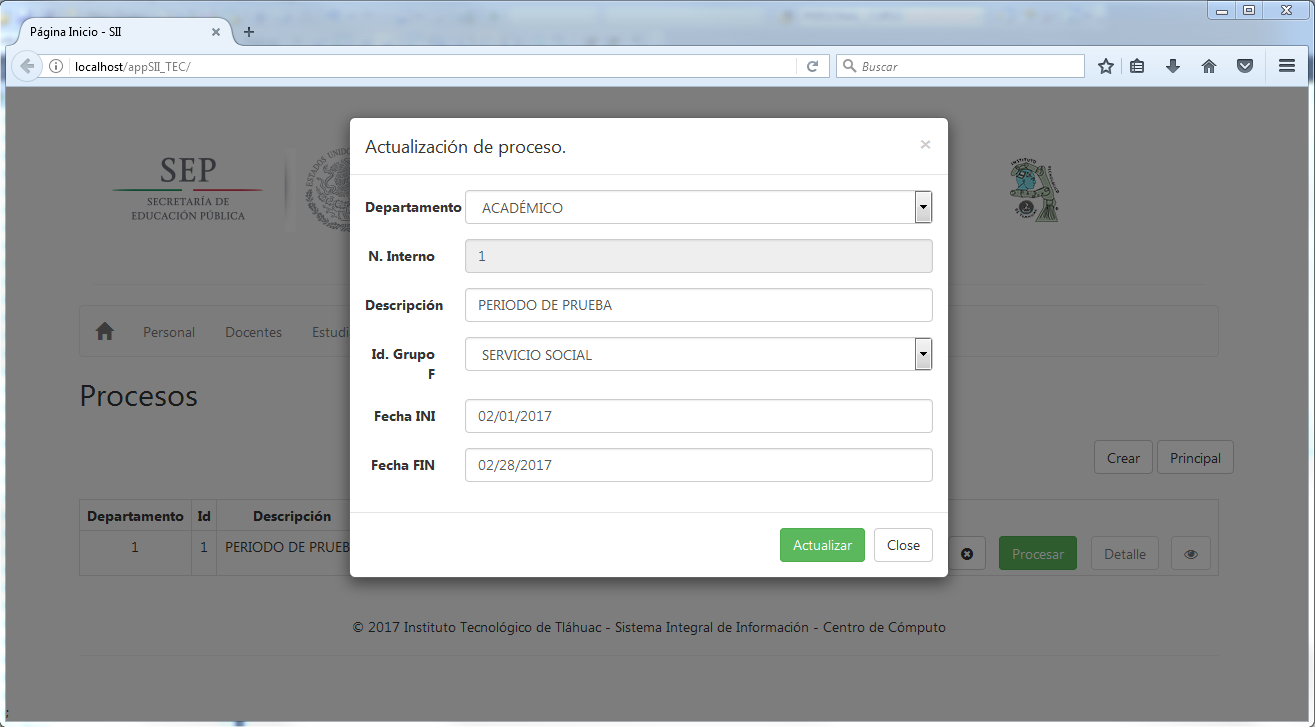
\includegraphics[width=16cm, height=9.5cm]{figuras/ProcesoActualiza}
		        \caption{Ventana emergente de actualizaci\'on de periodos de indicadores.}
		        \label{fig_ProcesoActualiza}
		    \end{figure}

		    \subsection{Baja de procesos}

		    En esta prueba prueba se muestra en la figura \ref{fig_FormulasElimina} la ventana emergente mostrada al momento de querer eliminar un proceso, el sistema pregunta al usuario si esta seguro de eliminar este registr\'o.\\

		    \begin{figure}[]
		        \centering
		        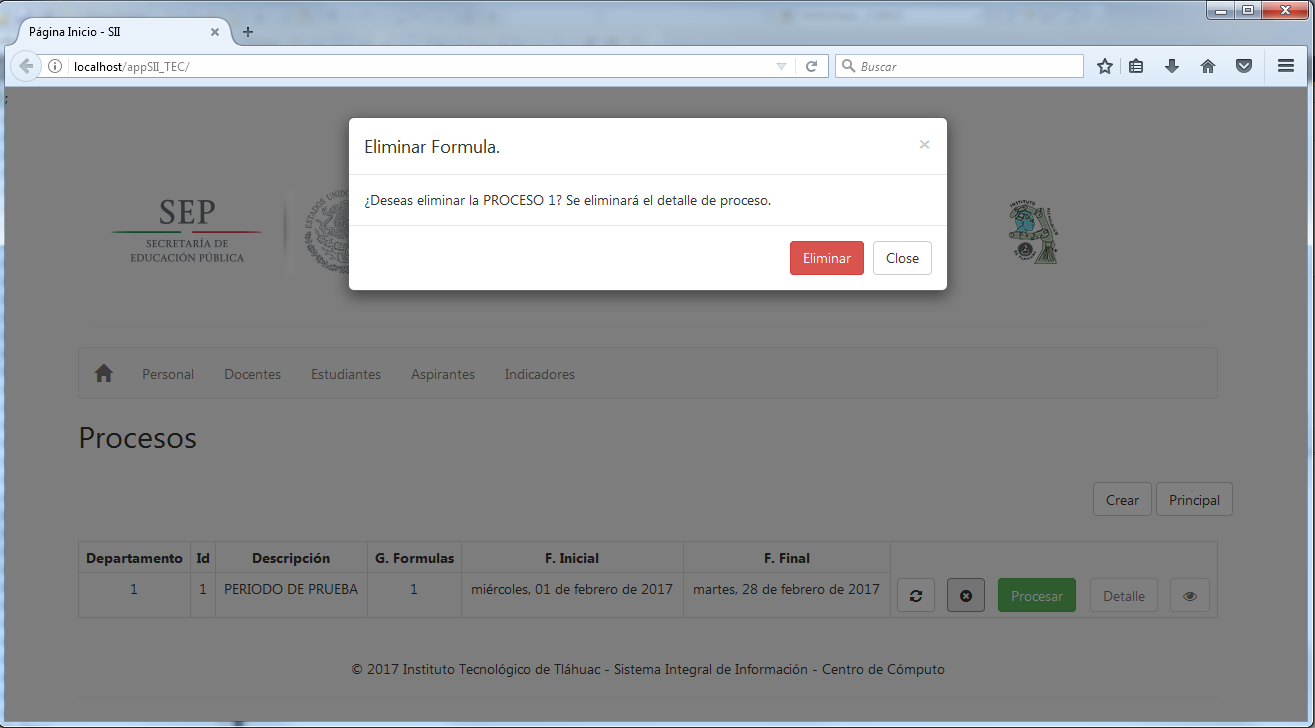
\includegraphics[width=16cm, height=9.5cm]{figuras/ProcesoElimina}
		        \caption{Mensaje de advertencia al eliminar un periodo de indicadores.}
		        \label{fig_ProcesoElimina}
		    \end{figure}

		    \subsection{Proceso de periodo de indicadores}

		    Esta funcionalidad permite ejecutar el proceso que resolver\'a y calculara los resultados de los indicadores. Pasando por toda la configuraci\'on de los mismos al presionar el bot\'on de Procesar de cada uno de los periodos enlistados, el sistema resolver\'a cada una de las f\'ormulas agrupadas en la colecci\'on de f\'ormulas seleccionada.\\

			Los periodos de indicadores tienen dos estatus, uno cuando fue creado y otro cuando ya fue procesado. El primero muestra un bot\'on de color verde con la leyenda Procesar, esto indicando que el periodo no ha sido procesado anteriormente. Este se ilustra en la figura \ref{fig_ProcesoProcesar}.\\


		    \begin{figure}[]
		        \centering
		        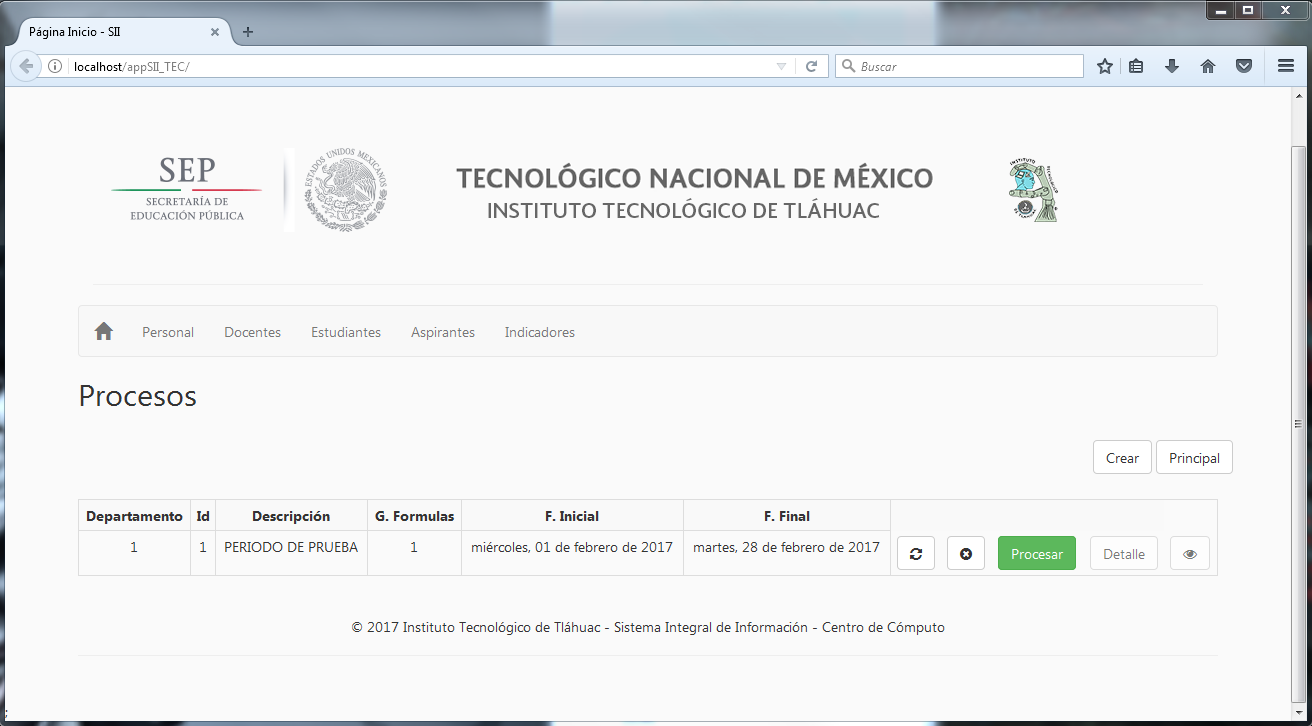
\includegraphics[width=16cm, height=9.5cm]{figuras/ProcesoProcesar}
		        \caption{Pantalla de procesos de indicadores listos para procesar.}
		        \label{fig_ProcesoProcesar}
		    \end{figure}

		    Cuando el periodo ya fue procesado, el bot\'on se mostrara de color rojo con la leyenda Reprocesar, el cual al presionarlo mostrara al usuario la leyenda indicando que ya existen datos para este periodo. Este mensaje se ilustra en la figura \ref{fig_ProcesoReprocesar}.\\

		    \begin{figure}[]
		        \centering
		        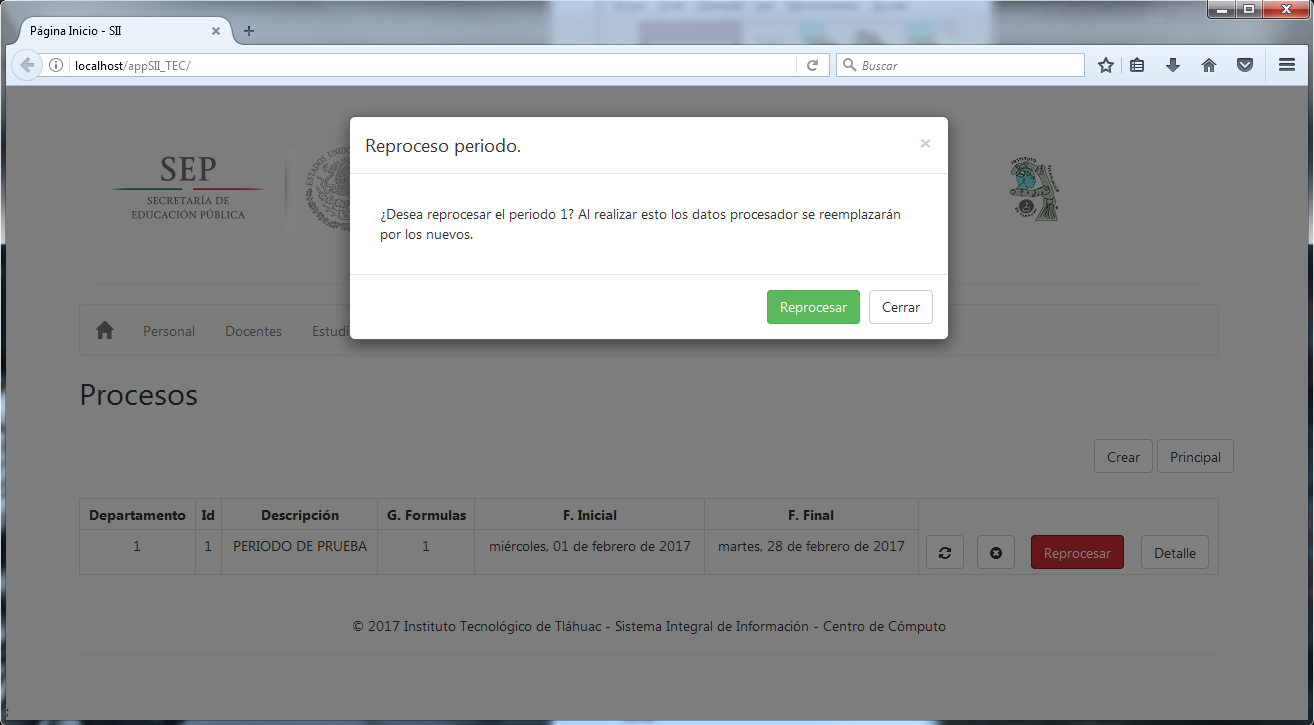
\includegraphics[width=16cm, height=9.5cm]{figuras/ProcesoReprocesar}
		        \caption{Alerta emergente con alerta de reproceso.}
		        \label{fig_ProcesoReprocesar}
		    \end{figure}

		    \subsection{Visualizaci\'on del detalle de procesos}

		   Al momento de procesar o reprocesar alg\'un periodo de indicadores, se podr\'a visualizar el detalle con los resultados del proceso. Esto se ilustra en la figura \ref{fig_ProcesoDetalle}.\\

		   \begin{figure}[]
		        \centering
		        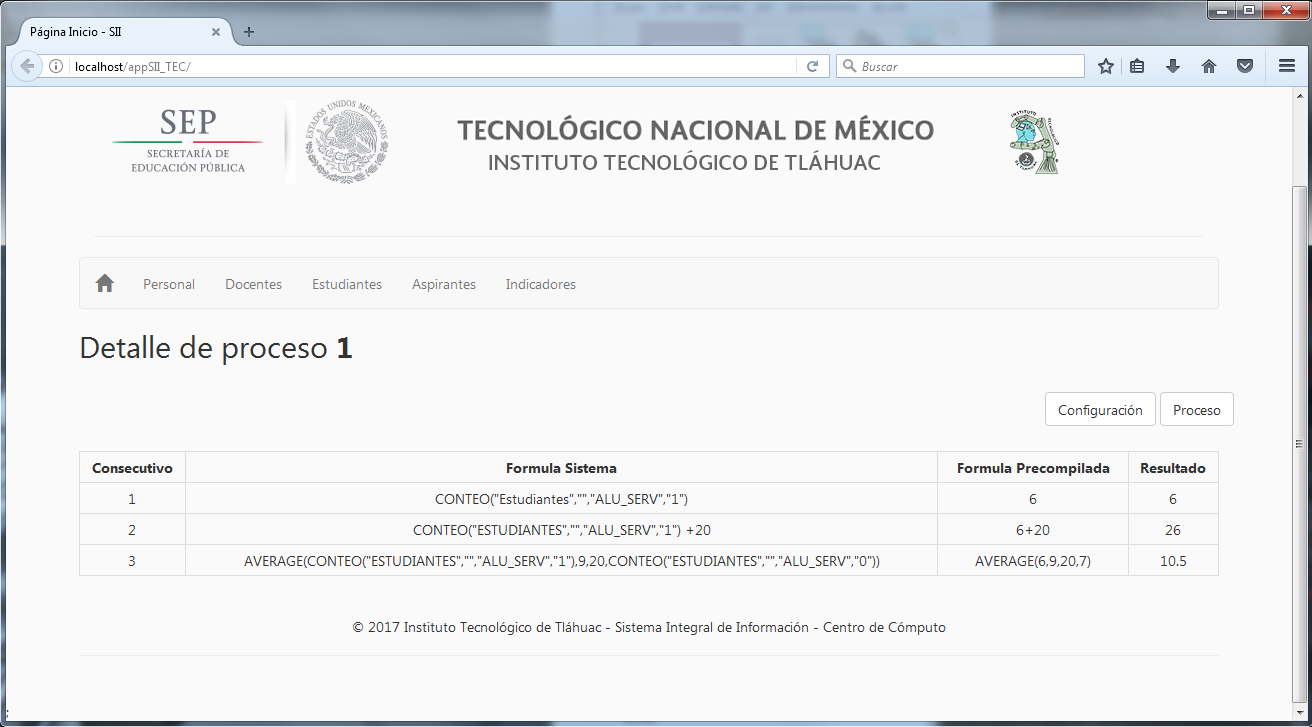
\includegraphics[width=16cm, height=9.5cm]{figuras/ProcesoDetalle}
		        \caption{Pantalla con el detalle de periodo de indicadores.}
		        \label{fig_ProcesoDetalle}
		    \end{figure}

		    El detalle de indicadores muestra datos que nos permiten realizar un mejor an\'alisis y seguimiento de los datos procesaros, ya que muestra las etapas por las que las f\'ormulas fueron avanzando par a lo largo del proceso. Esto es \'util cuando existe alg\'un error y se quisiera analizar en qu\'e parte de la f\'ormula se encuentra el error.\\

		    Con la visualizaci\'on del resultado del proceso de un periodo de indicadores se concluyen las pruebas del sistema.\\










